\section{Active Learning for Imbalanced Data Classification}
\label{al_for_imbalanced_data}
As we outlined in Section~\ref{sec:background}, active learning is primarily considered as a technique to reduce the number of training samples that need to be labeled for a classification task. From a traditional perspective, the active learner has access to a vast pool of unlabeled examples, and it aims to make a clever choice to select the most informative example to obtain its label. However, even in the cases where the labels of training data are already available, active learning can still be leveraged to obtain the informative examples through training sets \cite{Schohn_2000,Bordes_2005,Huang_2006}. For example, in large-margin classifiers such as Support Vector Machines (SVM), the \textit{informativeness} of an example is synonymous with its distance to the hyperplane. The farther an example is to the hyperplane, the more the learner is confident about its true class label, hence there is little, if any, benefit that the learner can gain by asking for the label of that example. On the other hand, the examples close to the hyperplane are the ones that yield the most information to the learner. Therefore, the most commonly used active learning strategy in SVMs is to check the distance of each unlabeled example to the hyperplane and focus on the examples that lie closest to the hyperplane, as they are considered to be the most informative examples to the learner.

\begin{figure}[t!]
    \centering
        \scalebox{0.5}{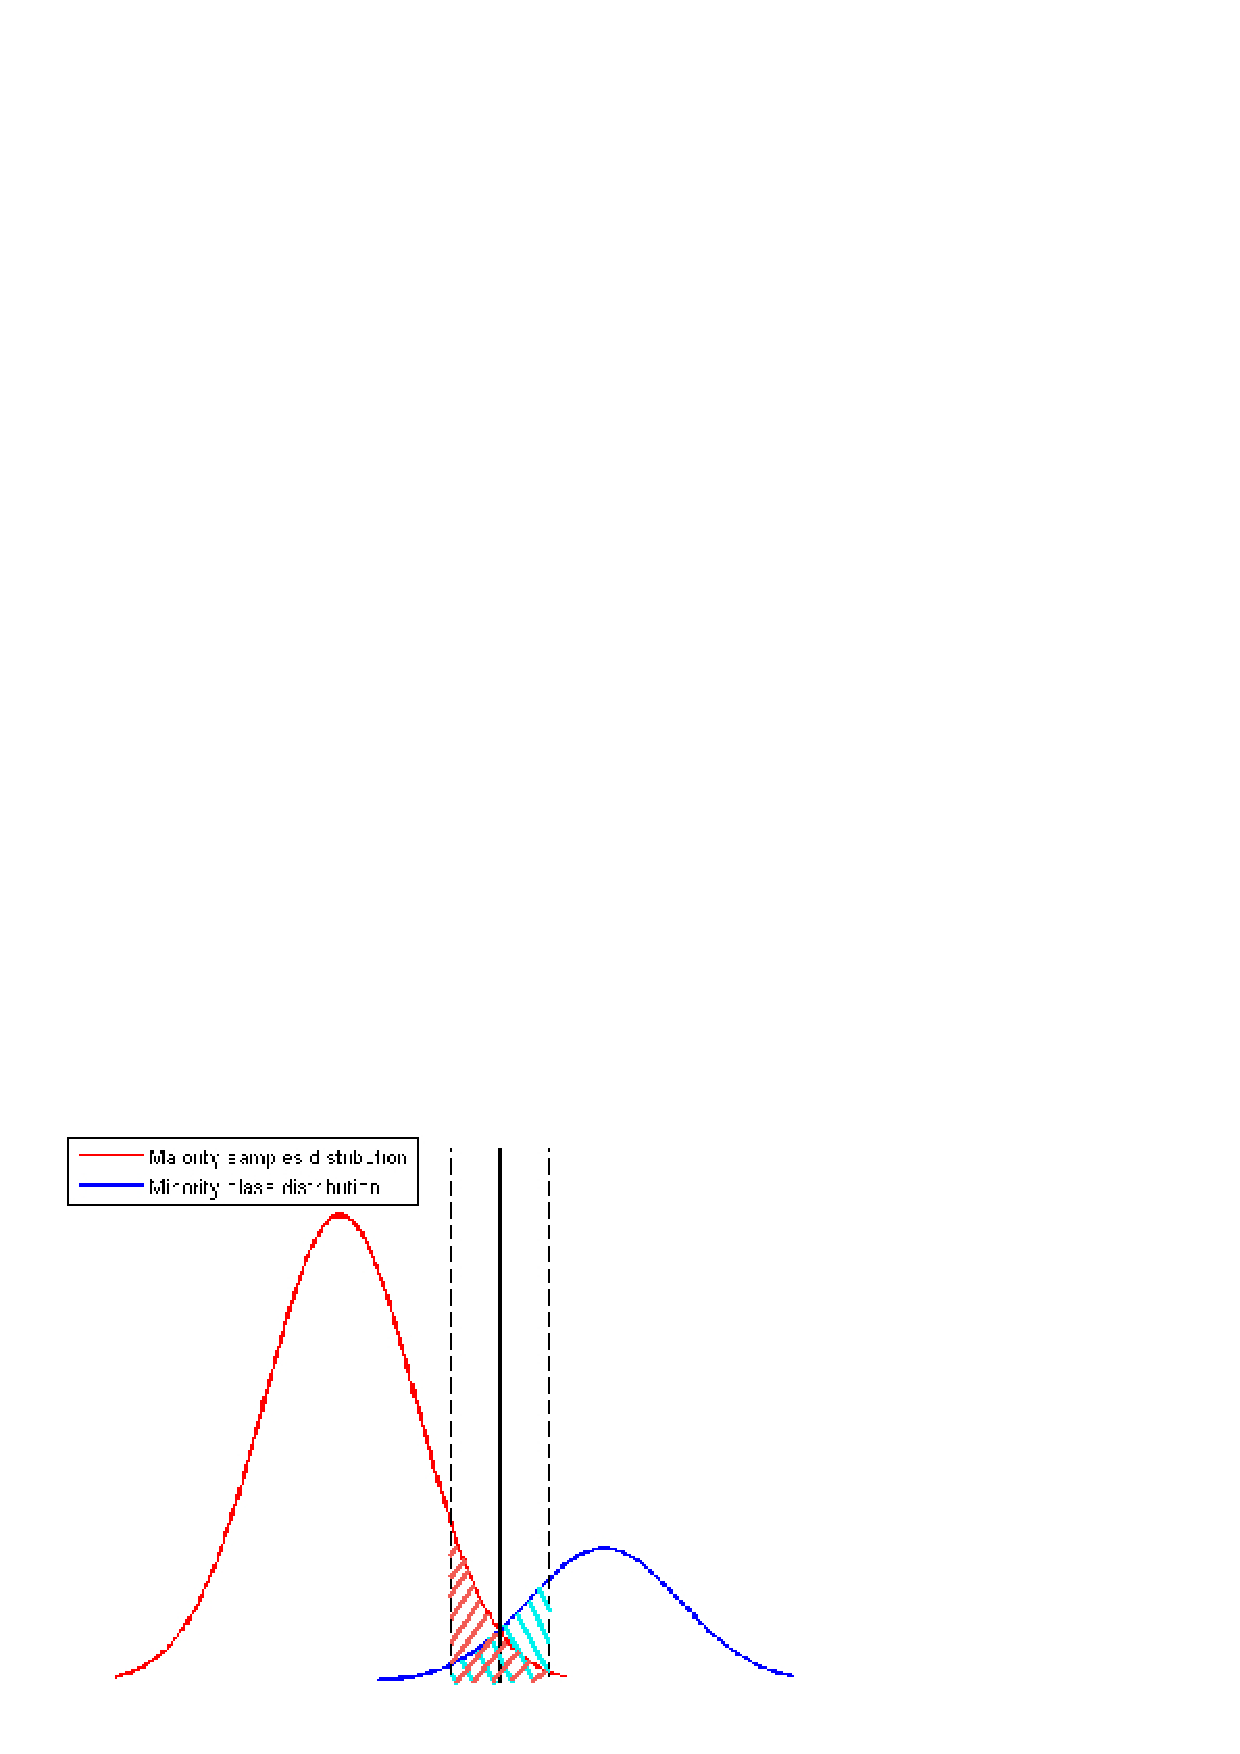
\includegraphics{Figures/lotb/al-imb-shade.pdf}}
    \caption{Data within the margin is less imbalanced than the entire data.}
    \label{fig:alimbshade}
\end{figure}

The strategy of selecting examples within the margin also strongly addresses the problems that arise from imbalanced classes. Suppose that the class distributions of an imbalanced dataset is given in Figure \ref{fig:alimbshade}. The shaded region corresponds to the class distribution of the data within the margin. As shown in the figure, the imbalance ratio of the classes within the margin is much smaller than the class imbalance ratio of the entire dataset. Therefore, any selection strategy that focuses on the examples in the margin most likely ends up with a more balanced class distribution than that of the entire dataset. Our empirical findings with various type of real-world data confirm that the imbalance ratios of the classes within the margin in real-world data are generally much lower than that of the entire data.

In this section, we constrain our discussion to standard two-class classification problems with Support Vector Machines (SVMs). The next section presents a brief overview of SVMs, followed by the working principles of an efficient active learning algorithm in Section \ref{ALpools}. We explain the advantage of using online SVMs with the active sample selection in Section \ref{LASVM}. In Section \ref{ES}, we then describe an early stopping heuristics for active learning.

\subsection{Support Vector Machines}
\label{SVMs}
Support Vector Machines \cite{Vapnik_1995} are well known for their strong theoretical foundations, generalization performance and ability to handle high dimensional data. In the binary classification setting, let $((x_{1}, y_{1})\cdots(x_{n}, y_{n}))$ be the training dataset where $x_i$ are the feature vectors representing the instances and  $y_i \in (-1,+1)$ be the labels of the instances.  Using the training set, SVM builds an optimum hyperplane -- a linear discriminant in a higher dimensional feature space -- that separates the two classes by the largest margin. This hyperplane is obtained by minimizing the following objective function:
\begin{equation}
\label{svm_primal}
\min_{{\bf{w}, b, \xi_{i}}}\frac{1}{2} {\bf w\cdot w}^T + C\sum_{i=1}^{N}\xi_i  \\
\end{equation}
\begin{equation}
\mbox{subject to}\left\{ \begin{array}{l} \forall i \; y_i({\bf
w}^T{\Phi(x_i)} - b)\geq 1-\xi_{i}\\ \forall i \; \xi_{i} \geq 0
\end{array} \right.
\end{equation}
where \textbf{w} is the norm of the hyperplane, $b$ is the  offset, $y_i$ are the labels, $\Phi(\cdot)$ is the mapping from input space to feature space, and $\xi_i$ are the slack variables that permit the non-separable case by allowing misclassification of training instances. In practice the convex quadratic programming (QP) problem in (\ref{svm_primal}) is solved by optimizing the dual cost function. The dual representation of (\ref{svm_primal}) is given as
\begin{equation}
\label{svm_dual}
\max W(\alpha) \equiv \sum_{i=1}^{N}\alpha_{i} - \frac{1}{2}\sum_{i,j}\alpha_i\alpha_{j}y_{i}y_{j}K({\bf x_i},{\bf x_j}) \\
\end{equation}
\begin{equation}
\mbox{subject to}\left\{ \begin{array}{l} \forall i\; 0 \leq \alpha_i \leq C\\ \sum_{i=1}^{N}\alpha_i y_i=0 \end{array} \right.
\end{equation}
where $y_i$ are the labels, $\Phi(\cdot)$ is the mapping from the input space to the feature space, $K({\bf x_i}, {\bf x_j})=\langle\Phi({\bf x_i}),\Phi({\bf x_j})\rangle$ is the kernel matrix and the $\alpha_i$'s are the \textit{Lagrange multipliers} which are non-zero only for the training instances which fall in the margin. Those training instances are called \textit{support vectors} and they define the position of the hyperplane. After solving the QP problem, the norm of the hyperplane \textbf{w} can be represented as
\begin{equation}
\label{svm_norm}
\textbf{w}=\sum_{i=1}^{n}\alpha_i\Phi(x_i)
\end{equation}

\subsection{Margin-based Active Learning with SVMs}
\label{ALpools}
Note that in (\ref{svm_norm}), only the support vectors affect the SVM solution. This means that if SVM is retrained with a new set of data which only consist of those support vectors, the learner will end up finding the same hyperplane. This emphasizes the fact that not all examples are equally important in training sets. Then the question becomes how to select the most informative examples for labeling from the set of unlabeled training examples. This section focuses on a form of selection strategy called \textit{margin-based active learning}. As we highlighted earlier, in SVMs the most informative example is believed to be the closest one to the hyperplane since it divides the \textit{version space} into two equal parts. The aim is to reduce the version space as fast as possible to reach the solution faster in order to avoid certain \textit{costs} associated with the problem. For the possibility of a non-symmetric version space, there are more complex selection methods suggested by \cite{Tong_2002}, but it has been observed that the advantage of those are not significant, considering their high computational costs.

\textbf{Active Learning with Small Pools:}
 The basic working principle of margin-based active learning with SVMs is: $i)$ train an SVM on the existing training data, $ii)$ select the closest example to the hyperplane, and $iii)$ add the new selected example to the training set and train again. In classical active learning \cite{Tong_2002}, the search for the most informative example is performed over the entire dataset. Note that, each iteration of active learning involves the recomputation of each training example's distance to the new hyperplane. Therefore, for large datasets, searching the entire training set is a very time consuming and computationally expensive task.

One possible remedy for this performance bottleneck is to use the ``59 trick'' \cite{Smola_2000}, which does not necessitate a full search through the entire dataset but locates an approximate most informative sample by examining a small constant number of randomly chosen samples. The method picks $L$ ($L \ll$ \# training examples) random training samples in each iteration and selects the best (closest to the hyperplane) among them. Suppose, instead of picking the closest example among all the training samples $X_N=(x_1, x_2, \cdots ,x_N)$ at each iteration, we first pick a random subset $X_L$, $L\ll N$ and select the closest sample $x_i$ from $X_L$ based on the condition that $x_i$ is among the top $p\%$ closest instances in $X_N$ with probability $(1-\eta)$. Any numerical modification to these constraints can be met by varying the size of $L$, and is independent of $N$. To demonstrate, the probability that at least one of the $L$ instances is among the closest $p\%$ is $1-(1-p\%)^L$. Due to the requirement of $(1-\eta)$ probability, we have
\begin{equation}
1-(1-p\%)^L = 1-\eta
\end{equation}
which follows the solution of $L$ in terms of $\eta$ and $p$
\begin{equation}
L={{\log \eta} \;/\;{\log(1-p\%)}}
\end{equation}
For example, the active learner will pick one example, with $95\%$ probability, that is among the top $5\%$ closest instances to the hyperplane, by randomly sampling only $\lceil \log(.05)/\log(.95) \rceil = 59$ examples regardless of the training set size. This approach scales well since the size of the subset $L$ is independent of  the training set size $N$, requires significantly less training time and does not have an adverse effect on the classification performance of the learner.

\begin{figure*}[t]
    \centering
        \scalebox{0.34}{\includegraphics{Figures/lotb/rpal.pdf}}
    \caption{Comparison of PRBEP and g-means of RS, AL(full search) and AL(random pool). The training times of AL(full search) vs. AL(random pool) until saturation in seconds are: 272 vs. 50 (grain), 142 vs. 32 (ship) and 126 vs. 13 (USPS). AL(random pool) is 4 to 10 times faster than AL(full search) with similar prediction performance.}
    \label{fig:rpal}
\end{figure*}

Figure \ref{fig:rpal} shows the comparisons of PRBEP and g-means performances of AL(random pool) and the traditional active learning method AL(full search) \cite{Tong_2002}. For the random pool strategy, we set $L=59$ which means we pick 59 random examples to form the query pool  at each learning step and pick the closest example to the hyperplane from this pool. RS corresponds to the random sampling strategy where the examples are selected randomly. As Figure \ref{fig:rpal} depicts, active learning method with small pools achieves as good prediction performance as the traditional active learning method. Moreover, the random pool strategy is 4 to 10 times faster than traditional active learning for the given datasets.

\subsection{Online SVM for Active Learning}
\label{LASVM}
Online learning algorithms are usually associated with problems where the complete training set is not available. However, in cases where the complete training set is available, their computational properties can be leveraged for faster classification and incremental learning. In our framework, we use an online SVM algorithm, LASVM \cite{Bordes_2005} instead of a traditional batch SVM tool (e.g., libsvm, SVM\textsuperscript{\textit{light}}). LASVM is an online kernel classifier which relies on the traditional soft margin SVM formulation. LASVM yields the classification accuracy rates of the state-of-the art traditional SVM solvers but requires less computational resources. Traditional SVM works in a batch setting where all the training instances are used to form the one and final model. LASVM, on the other hand, works in an online setting, where its model is continually modified as it processes training instances one by one. Each LASVM iteration receives a fresh training example and tries to optimize the dual cost function in Equation (\ref{svm_dual}) using feasible direction searches.
They can select a new data to process either by random or active selection and can integrate the information of the new seen data to the system without training on all the samples again, hence they can incrementally build a learner. This working principle of online learning algorithms leads to speed improvement and less memory demand which makes the algorithm applicable to very large datasets. More importantly, this incremental working principle suits the nature of active learning in a much better way than the batch algorithms. Empirical evidence indicates that a single presentation of each training example to the algorithm is sufficient to achieve training errors comparable to those achieved by the SVM solution \cite{Bordes_2005}. In section \ref{ES} we also show that if we use an early stopping criteria in active sample selection, we do not have to introduce all training examples to the learner.

\subsection{Active Learning with Early Stopping}
\label{ES}
Early stopping criteria is advantageous to active learning since it converges to the solution faster than the random sample selection method. A theoretically sound method to stop training is when the examples in the margin are exhausted. To check if there are still unseen training examples in the margin, the distance of the new selected example is compared against the support vectors of the current model. If the new selected example by active learning (closest to the hyperplane) is not closer than any of the support vectors, we conclude that the margin is exhausted. A practical implementation of this idea is to count the number of support vectors during the active learning training process. If the number of the support vectors stabilizes, it implies that all possible support vectors have been selected by the active learning method.

\begin{figure}[b]
    \hspace{-10mm}
        \scalebox{0.3}{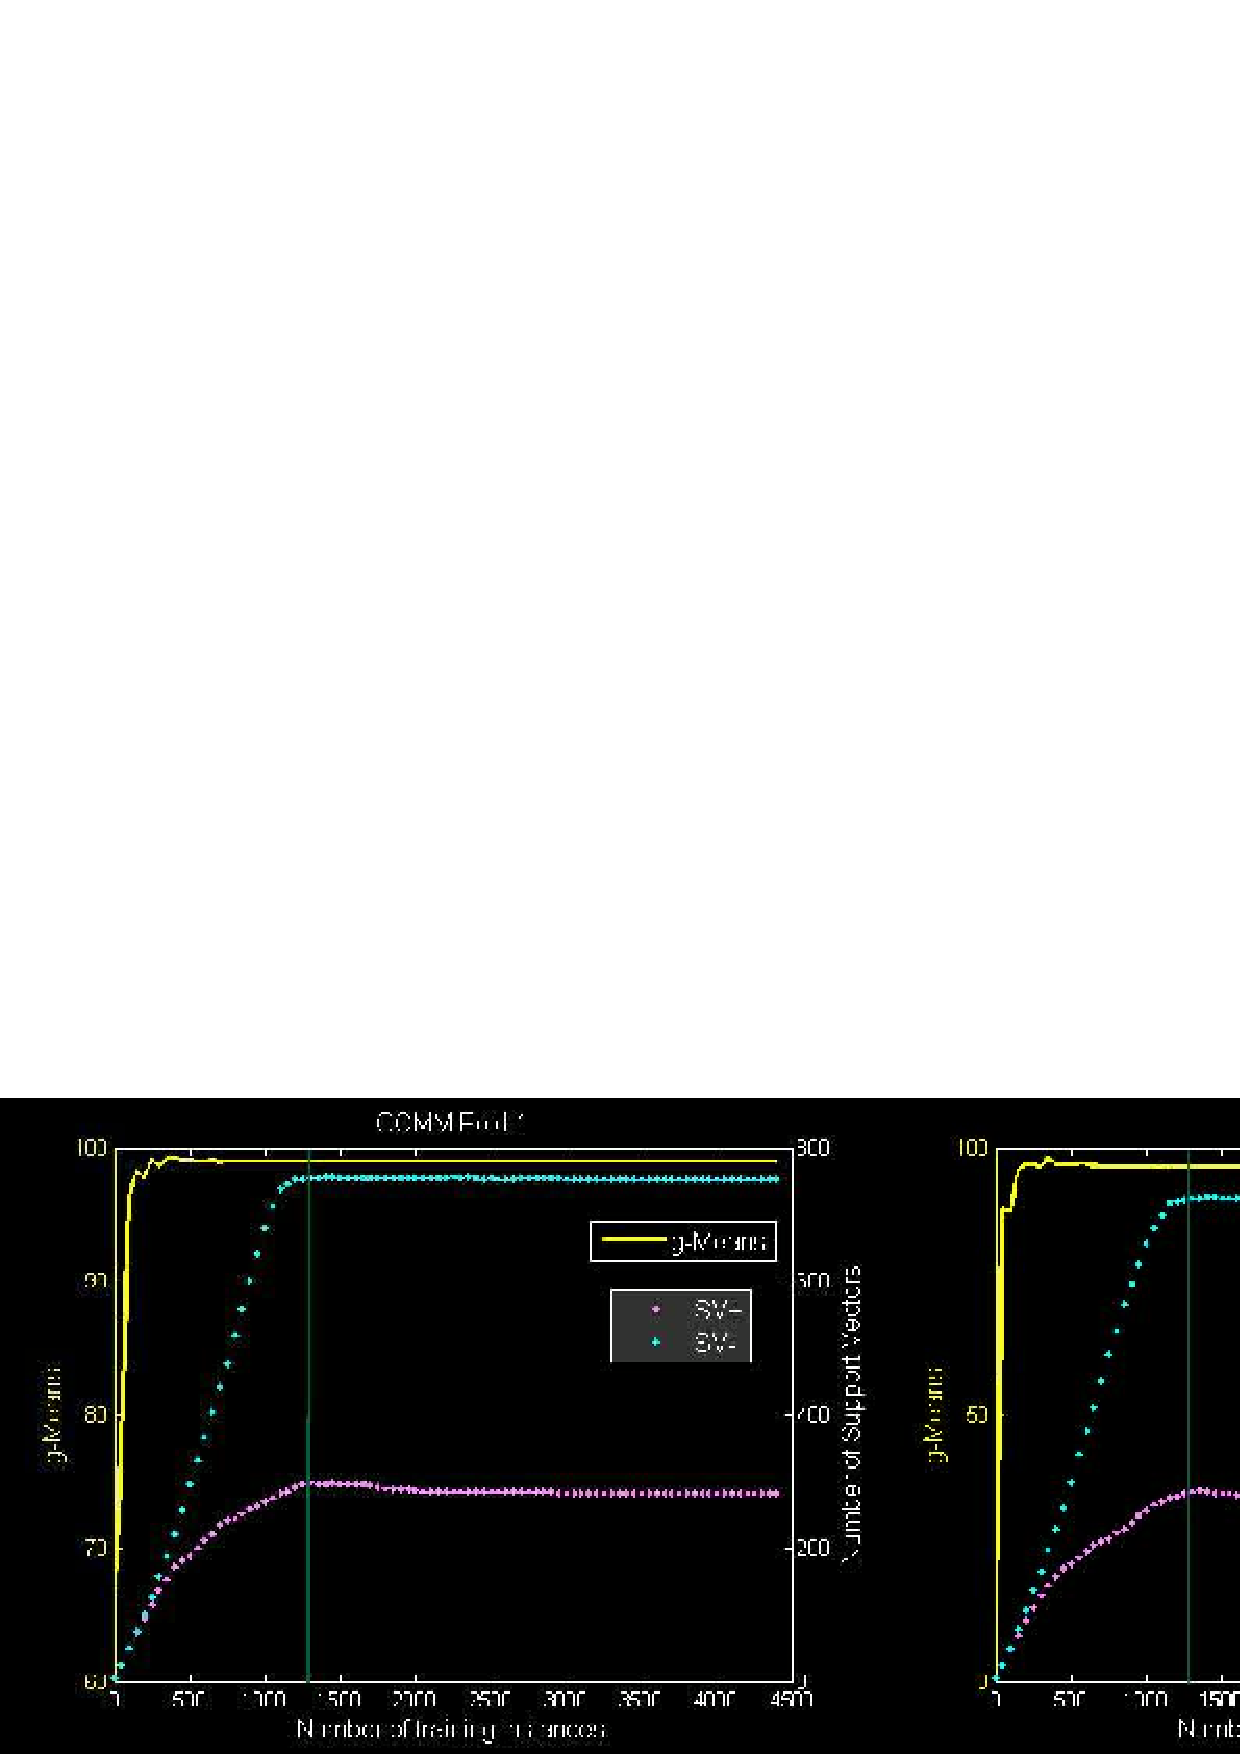
\includegraphics{Figures/lotb/comm.pdf}}
    \caption{3-fold cross-validation results for the training set of the category COMM in CiteSeer dataset. Vertical lines correspond to early stopping points.}
    \label{fig:comm}
\end{figure}

In order to analyze this method, we conducted a 3-fold cross-validation on one of the datasets (see Figure \ref{fig:comm}). In cross-validation, $2/3$ of the training set is used for training and the remaining $1/3$ is reserved as the hold-out dataset. Since the training set distribution is representative of the test set distribution, we believe that the algorithm's behavior would most likely be the same in the test set. As can be seen in Figure \ref{fig:comm}, in active learning setups, after using certain number of labeled training data, the number of support vectors saturates and  g-means levels off as well. Those graphs support the idea that the model does not change after the system observes enough informative samples. Further, adding more training data after this point does not make a remarkable change in the model and consequently in prediction performance. Notice that in Figure \ref{fig:comm} the vertical line indicates the suggested early stopping point and it is approximately equal in all three folds. As a result, we adopt the early stopping strategy of examining the number of support vectors in the entire training datasets without performing cross-validation.

\subsection{Performance Metrics}
Classification accuracy is not a good metric to evaluate classifiers in applications with class imbalance problem.  SVMs have to achieve a tradeoff between maximizing the margin and minimizing the empirical error. In the non-separable case, if the misclassification penalty $C$ is very small, SVM learner simply tends to classify every example as negative. This extreme approach makes the \textit{margin} the largest while making no classification errors on the negative instances. The only error is the cumulative error of the positive instances which are already few in numbers. Considering an imbalance ratio of 99 to 1, a classifier that classifies everything as negative, will be 99\% accurate but it will not have any practical use as it can not identify the positive instances.

For the evaluation of our results, we use several other prediction performance metrics such as g-means, AUC and PRBEP which are commonly used in imbalanced data classification. g-means \cite{Kubat_1997} is denoted as $g=\sqrt{sensitivity \cdot specificity}$ where sensitivity is the accuracy on the positive instances given as $True Pos./(True Pos.+False Neg.)$ and specificity is the accuracy on the negative instances given as $True Neg./(True Neg.+False Pos.)$.

The Receiver Operating Curve (ROC) displays the relationship between sensitivity and specificity at all possible thresholds for a binary classification scoring model, when applied to independent test data. In other words, ROC curve is a plot of the true positive rate against the false positive rate as the decision threshold is changed. The \textit{area under the ROC curve} (AUC) is a numerical measure of a model's discrimination performance and shows how successfully and correctly the model separates the positive and negative observations and ranks them. Since AUC metric evaluates the classifier across the entire range of decision thresholds, it gives a good overview about the performance when the operating condition for the classifier is unknown or the classifier is expected to be used in situations with significantly different class distributions.

Precision Recall Break-Even Point (PRBEP) is another commonly used performance metric for imbalanced data classification. PRBEP is the accuracy of the positive class at the threshold where precision equals to recall. Precision is defined as $True Pos./(True Pos.+False Pos.)$ and recall is defined as $True Pos./(True Pos.+False Neg.)$


\begin{table}[t!]
\caption{Overview of the datasets.} \centering \small
\begin{tabular}{l|l|r@{\hspace{2mm}}r@{\hspace{2mm}}r@{\hspace{2mm}}r|c c}
\hline
\multicolumn{2}{c|}{Dataset}&\#Feat.&\#Pos&\#Neg&Ratio&c&$\gamma$\\
\hline\hline
\multirow{5}{5mm}{\begin{sideways}\parbox{13mm}{Reuters}\end{sideways}}&Crude&8315&389&7381&19.0&2&1\\
&Grain&8315&433&7337&16.9&2&1\\
&Interest& 8315 &347&7423&21.4&1&2\\
&Money-fx& 8315 &538&7232&13.4&1&0.5\\
&Ship& 8315 &197&7573&38.4&1&0.5\\
&Wheat& 8315 &212&7558&35.7&1&0.5\\
\hline
\multirow{5}{5mm}{\begin{sideways}\parbox{12mm}{CiteSeer}\end{sideways}}
&AI& 6946 &1420&5353&4.3&50&0.1\\
&COMM& 6946 &1252&5341&4.2&50&0.1\\
&Crypt& 6946 &552&6041&11.0&50&0.1\\
&DB& 6946 &819&5775&7.1&50&0.1\\
&OS& 6946 &262&6331&24.2&50&0.1\\
\hline
\multirow{2}{5mm}{\begin{sideways}\parbox{8mm}{UCI}\end{sideways}}
&Abalone-7& 9 &352&3407&9.7&100&0.01\\
&Letter-A&16 &710&17290&24.4&10&0.01\\
&Satimage&36&415&4020&9.69&50&0.001\\
\hline
\multicolumn{2}{c|}{USPS}& 256 &1232&6097&5.0&1000&2\\
\hline
\multicolumn{2}{c|}{MNIST-8}& 780 &5851&54149&9.3&1000&0.02\\
\hline
\end{tabular}
\label{tbl:overview}
\end{table}

\subsection{Datasets}
We study the performance of the algorithm on various benchmark real-world datasets. The overview of the datasets are given in Table \ref{tbl:overview}. The \emph{Reuters-21578} is a popular text mining benchmark dataset. We test the algorithms with 8 of the top 10 most populated categories of \emph{Reuters-21578}. We did not use categories `earn' and `acq' since their class imbalance ratios are not high enough. As a text dataset, we also used 5 categories from CiteSeer\footnote{http://citeseer.ist.psu.edu} data. We used 4 benchmark datasets from the popular UCI Machine Learning Repository as well. \emph{Letter} and \emph{satimage} are image datasets. The `letter A' is used as the positive class in \emph{letter} and `class 4' (damp grey soil) is used as positive class in \emph{satimage}. \emph{Abalone} is a biology dataset where the instances labeled as `class 7' are used to form the positive class. \emph{MNIST} and \emph{USPS} are OCR data of handwritten digits and `digit 8' is used as a positive class in \emph{Mnist}. \emph{Adult} is a census dataset to predict if the income of a person is greater than 50K based on several census parameters, such as age, education, marital status etc. The training set consists of 32,562 instances and the class imbalance ratio is 3. \emph{Waveform} is a popular artificial dataset used commonly in simulation studies. These datasets cover a wide range of data imbalance ratios.

\subsection{Experiments and Empirical Evaluation}
\label{lotb_experiments}
We first conduct experiments to compare the performance of AL(random pool) strategy with the traditional active learning method, AL(full search). The results show that with the proposed method, we can make faster active learning without sacrificing any prediction performance (see Figure \ref{fig:rpal}). In the rest of the section, we refer to AL(random pool) as AL since it is the only active learning method that we used afterwards.

\begin{figure}[b!]
        \scalebox{0.47}{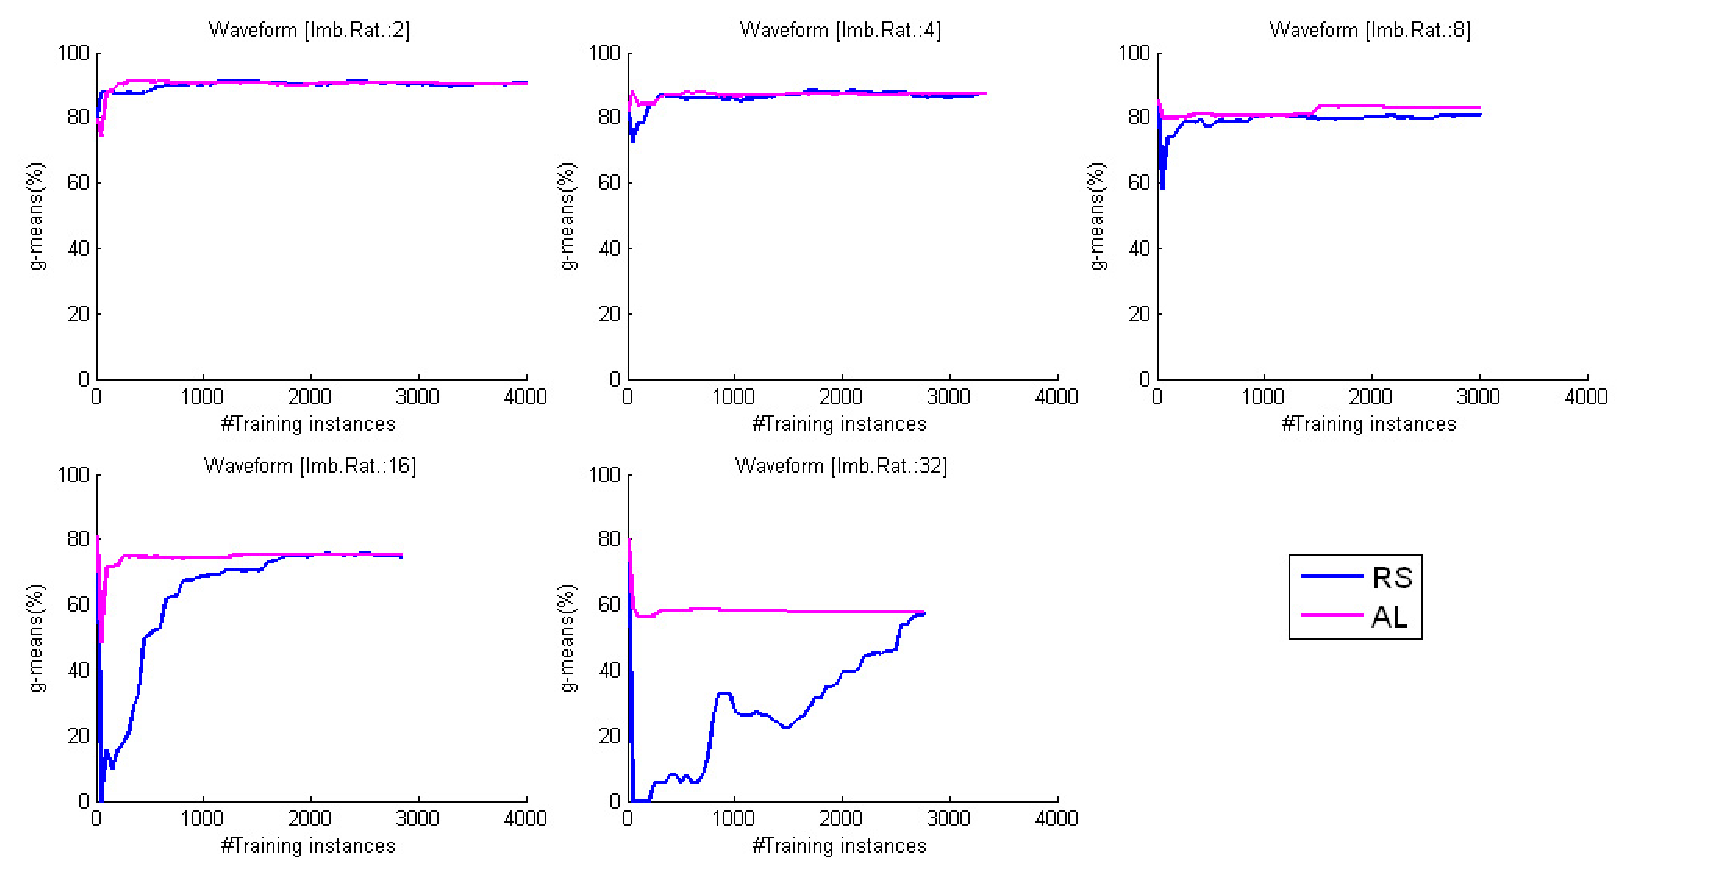
\includegraphics{Figures/lotb/wfall.eps}}
    \caption{Comparison of g-means of AL and RS on the waveform datasets with different imbalance ratios (Imb.R.=2, 4, 8, 16, 32).}
    \label{fig:wfall}
\end{figure}
\begin{figure}[bh!]
\begin{center}
\vspace{-4mm}
\subfigure {
\includegraphics[width=55mm]{Figures/lotb/adultall_1.jpg}
}
\subfigure {
\includegraphics[width=55mm]{Figures/lotb/adultall_2.jpg}
}\\
\vspace{-2mm}
\subfigure {
\includegraphics[width=55mm]{Figures/lotb/adultall_3.jpg}
}
\subfigure {
\includegraphics[width=55mm]{Figures/lotb/adultall_4.jpg}
}
 \caption{Comparison of PRBEP of AL and RS on the adult datasets with different imbalance ratios (Imb.R.=3, 10, 20, 30).}
    \label{fig:adultall}
\end{center}
\end{figure}


In order to make a thorough analysis on the effect of AL to imbalanced data classification, we examine its performance by varying class imbalance ratios using two performance metrics. We randomly remove the examples from the minority class in \emph{Waveform} and \emph{Adult} datasets to achieve different data imbalance ratios. Comparisons of g-means of AL and RS in Figure \ref{fig:wfall} show that the prediction performance of AL is less sensitive to the class imbalance ratio changes than that of the RS. Comparisons of another performance metric PRBEP in Figure \ref{fig:adultall} give even more interesting results. As the class imbalance ratio is increased, AL curves display peaks in the early steps of the learning. This implies that by using an early stopping criteria AL can give higher prediction performance than RS can possibly achieve even after using all the training data. Figure \ref{fig:adultall} curves allow us to think that addition of any instances to the learning model after finding the informative instances can be detrimental to the prediction performance of the classifier. This finding strengthens the idea of applying an early stopping to active learning algorithms.

\begin{figure}[t!]
        \scalebox{0.3}{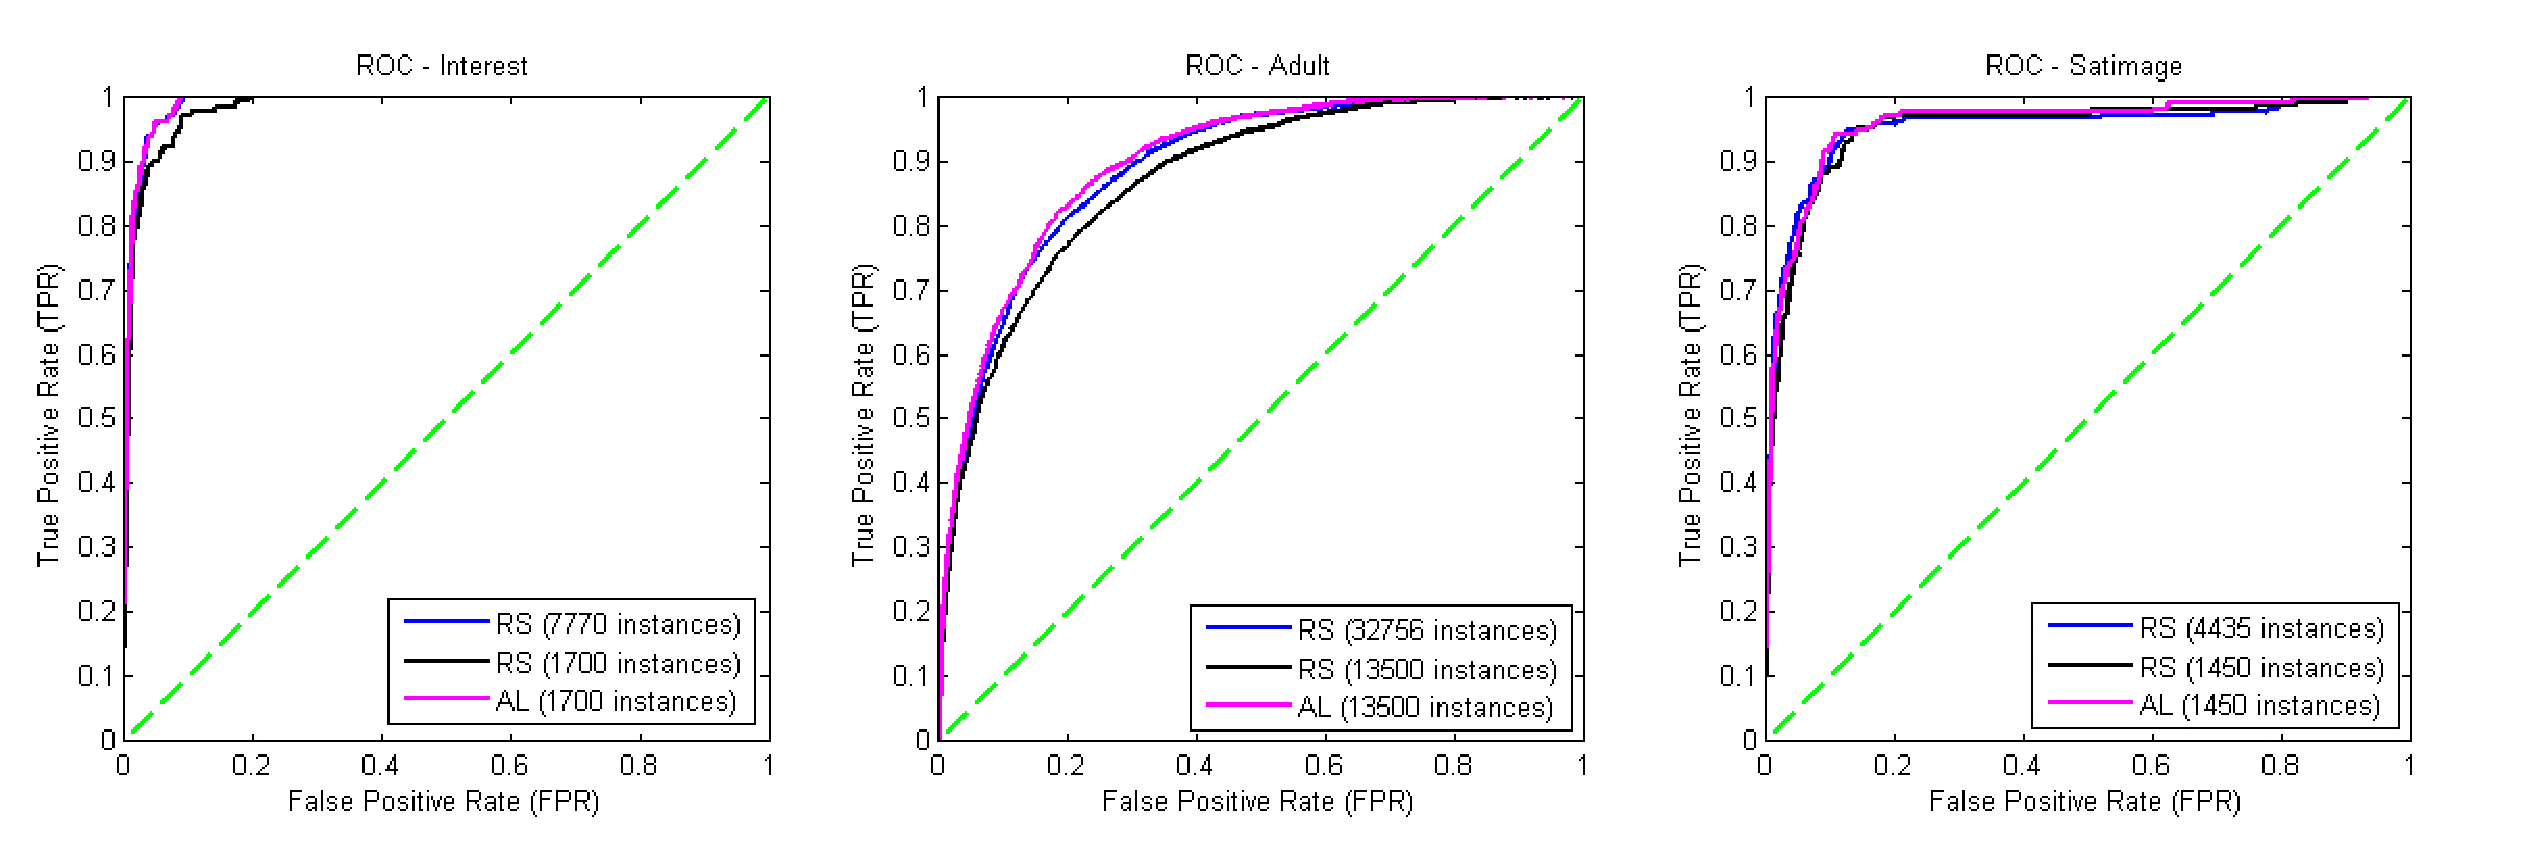
\includegraphics{Figures/lotb/rocall.eps}}
    \caption{Comparison of ROC curves of AL, RS (early stopped at the same number of instances as AL) and RS (with all training data) in Interest, Adult and Satimage datasets.}
    \label{fig:rocall}
\end{figure}
\begin{figure}[b!]
    \centering
        \scalebox{0.45}{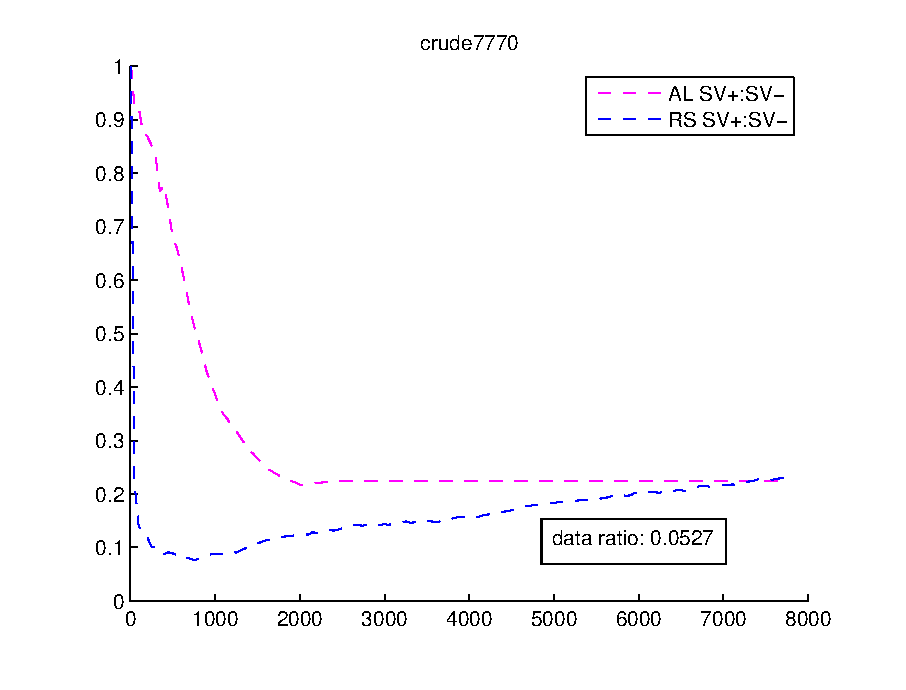
\includegraphics{Figures/lotb/cruderatio.eps}}
    \caption{Support Vector ratios in AL and RS}
    \label{cruderatio}
\end{figure}


We also compared the performance of early stopped AL with Batch algorithm. Table \ref{tbl:AUC} presents the g-means and the AUC values of the two methods. Data efficiency column for AL indicates that by processing only a portion of the examples from the training set, AL can achieve similar or even higher prediction performance than that of Batch which sees all the training examples. Another important observation from Table \ref{tbl:AUC} is that support vector imbalance ratios in the final models are much less than the class imbalance ratios of the datasets. This confirms our discussion of Figure \ref{fig:alimbshade}. The class imbalance ratio within the margins are much less than the class imbalance ratio of the entire data and active learning can be used to reach those informative examples which most likely become support vectors without seeing all the training examples.

In order to evaluate the methods at different thresholds, we also investigate the ROC curves as given in Figure \ref{fig:rocall}. The ROC curves of AL are similar and sometimes better than of the Batch algorithm (RS, seeing all the training examples). The AUC of AL and Batch are 0.8980 and 0.8910 respectively in the \emph{Adult} dataset. At the same number of training instances where AL is early stopped, AUC of RS can be substantially lower. As Figure \ref{fig:rocall} shows, the ROC curve of AL is markedly higher than that of RS (early stopping) and the AUC values are 0.8980 and 0.8725 respectively for \emph{Adult} dataset. These results suggest that AL converges faster than RS using fewer and informative instances and AL can get even higher prediction performance than the Batch algorithm by processing only a portion of the training set.

\begin{table*}[t!]\centering{
\caption{Comparison of g-means and AUC for AL and RS with entire training data (Batch).
Support vector ratios are given at the saturation point. Data efficiency corresponds to the percentage of training instances which AL processes to reach saturation.}
\begin{tabular}{l|l|r r|r r||r|r|c}
\hline
\multicolumn{2}{c|}{\multirow{2}{1cm}{Dataset}}
&\multicolumn{2}{c|}{g-means (\%)}
&\multicolumn{2}{c||}{AUC (\%)}
&Imb.&SV- /&\multirow{2}{12mm}{Data Efficiency}
\\
\cline{3-6}
\multicolumn{2}{c|}{}&Batch&AL&Batch&AL&Rat.&SV+\\
\hline\hline
\multirow{8}{1mm}{\begin{sideways}\parbox{12mm}{Reuters}\end{sideways}}
&Corn&85.55&86.59&99.95&99.95&41.9&3.13&11.6\%\\
&Crude&88.34&89.51&99.74&99.74&19.0&2.64&22.6\%\\
&Grain&91.56&91.56&99.91&99.91&16.9&3.08&29.6\%\\
&Interest&78.45&78.46&99.01&99.04&21.4&2.19&30.9\%\\
&Money-fx&81.43&82.79&98.69&98.71&13.4&2.19&18.7\%\\
&Ship&75.66&74.92&99.79&99.80&38.4&4.28&20.6\%\\
&Trade&82.52&82.52&99.23&99.26&20.1&2.22&15.4\%\\
&Wheat&89.54&89.55&99.64&99.69&35.7&3.38&11.6\%\\
\hline
\multirow{5}{1mm}{\begin{sideways}\parbox{12mm}{CiteSeer}\end{sideways}}
&AI&87.83&88.58&94.82&94.69&4.3&1.85&33.4\%\\
&COMM&93.02&93.65&98.13&98.18&4.2&2.47&21.3\%\\
&CRYPT&98.75&98.87&99.95&99.95&11.0&2.58&15.2\%\\
&DB&92.39&92.39&98.28&98.46&7.1&2.50&18.2\%\\
&OS&91.95&92.03&98.27&98.20&24.2&3.52&36.1\%\\
\hline
\multirow{3}{1mm}{\begin{sideways}\parbox{6mm}{UCI}\end{sideways}}
&Abalone-7&100.0&100.0&100.0&100.0&9.7&1.38&24.0\%\\
&Letter-A&99.28&99.54&99.99&99.99&24.4&1.46&27.8\%\\
&Satimage&82.41&83.30&95.13&95.75&9.7&2.62&41.7\%\\
\hline
\multicolumn{2}{c|}{USPS}&99.22&99.25&99.98&99.98&4.9&1.50&6.8\%\\
\hline
\multicolumn{2}{c|}{MNIST-8}&98.47&98.37&99.97&99.97&9.3&1.59&11.7\%\\
\hline
\end{tabular}
\label{tbl:AUC}

}
\end{table*}

In Figure \ref{cruderatio}, we investigate how the number of support vectors changes in AL and Random Sampling (RS). With random sampling, the instances are selected for the learner randomly from the entire pool of the training data. Therefore, the support vector imbalance ratio quickly approaches the data imbalance ratio. As learning continues, the learner should gradually see all the instances within the final margin and the support vector imbalance ratio decreases. At the end of training with RS, the support vector imbalance ratio is the data imbalance ratio within the margin. The support vector imbalance ratio curve of AL is drastically different than RS. AL intelligently picks the instances closest to the margin in each step. Since the data imbalance ratio within the margin is lower than data imbalance ratio, the support vectors in AL are more balanced than RS during learning. Using AL, the model saturates by seeing only 2000 (among 7770) training instances and reaches the final support vector imbalance ratio. Note that both methods achieve similar support vector imbalance ratios when learning finishes, but AL achieves this in the early steps of the learning.

We compare AL against several other strategies as well. Among them, undersampling (US), and an oversampling method (SMOTE) are examples of resampling techniques which require preprocessing. It has been shown that oversampling at random does not help to improve prediction performance \cite{Japkowicz_2002} therefore we use a more complex oversampling method, namely SMOTE.  Synthetic Minority Oversampling Technique (SMOTE) oversamples the minority class by creating synthetic examples rather than with replacement. The $k$ nearest positive neighbors of all positive instances are identified and synthetic positive examples are created and placed randomly along the line segments joining the $k$ minority class nearest neighbors.

\begin{table*}[t!]\centering{
\caption{Comparison of PRBEP and training time. }\small
\begin{tabular}{l|l|r r r r r|r r}
\hline
\multicolumn{2}{c|}{Metric}&\multicolumn{5}{c|}{PRBEP}&\multicolumn{2}{c}{Training time (sec.)}\\
\hline
\multicolumn{2}{c|}{Dataset}&Batch&US&SMOTE&DC&AL&SMOTE&AL\\
\hline
\hline
\multirow{8}{5mm}{\begin{sideways}\parbox{13mm}{Reuters}\end{sideways}}
&Corn&91.07&78.57&91.07&89.28&89.29&87&16\\
&Crude&87.83&85.70&87.83&87.83&87.83&129&41\\
&Grain&92.62&89.93&91.44&91.94&91.94&205&50\\
&Interest&76.33&74.04&77.86&75.57&75.57&116&42\\
&Money-fx&73.74&74.30&75.42&75.42&76.54&331&35\\
&Ship&86.52&86.50&88.76&89.89&89.89&49&32\\
&Trade&77.77&76.92&77.77&77.78&78.63&215&38\\
&Wheat&84.51&81.61&84.51&84.51&85.92&54&25\\
\hline
\multirow{5}{5mm}{\begin{sideways}\parbox{12mm}{CiteSeer}\end{sideways}}
&AI&78.80&80.68&78.99&78.79&79.17&1402&125\\
&COMM&86.59&86.76&86.59&86.59&86.77&1707&75\\
&CRYPT&97.89&97.47&97.89&97.89&97.89&310&19\\
&DB&86.36&86.61&86.98&86.36&86.36&526&41\\
&OS&84.07&83.19&84.07&84.07&84.07&93&23\\
\hline
\multirow{3}{5mm}{\begin{sideways}\parbox{6mm}{UCI}\end{sideways}}
&Abalone-7&100.0&100.0&100.0&100.0&100.0&16&4\\
&Letter-A&99.48&96.45&99.24&99.35&99.35&86&3\\
&Satimage&73.46&68.72&73.46&73.93&73.93&63&21\\
\hline
\multicolumn{2}{c|}{USPS}&98.44&98.44&98.13&98.44&98.75&4328&13\\
\hline
\multicolumn{2}{c|}{MNIST-8}&97.63&97.02&97.74&97.63&97.74&83,339&1,048\\
\hline

\end{tabular}
\label{tbl:results}
}
\end{table*}

As an algorithmic method to compare, we use the method of assigning different costs (DC) to the positive and negative classes as the misclassification penalty parameter. For instance, if the imbalance ratio of the data is 19:1 in favor of the negative class, the cost of misclassifying a positive instance is set to be 19 times greater than that of misclassifying a negative one. We use the online SVM package LASVM\footnote{Available at http://leon.bottou.org/projects/lasvm} in all experiments. Other than the results of the methods addressing class imbalance problem, we also give results of Batch algorithm with the original training set to form a baseline. LASVM is run in random sampling mode for US, SMOTE and DC.

We present the comparisons of the methods for g-means performance metric for several datasets in Figure \ref{eightgraphs}. The right border of the shaded pink area is the place where the aforementioned early stopping strategy is applied.  The curves in the graphs are averages of 10 runs. For completeness, we did not stop the AL experiments at the early stopping point but allow them to run on the entire training set. Table \ref{tbl:results} presents the PRBEP of the methods and the total running times of the SMOTE and AL on 18 benchmark and real-world datasets. The results for active learning in Table \ref{tbl:results} depict the results in the early stopping points. The results for the other methods in Table \ref{tbl:results} depict the values at the end of the curves --when trained with the entire dataset-- since those methods do not employ any early stopping criteria. We did not apply early stopping criteria to the other methods because as observed from Figure \ref{eightgraphs}, no early stopping criteria would achieve a comparable training time with of AL's training time without a significant loss in their prediction performance based on convergence time. The other methods converge to similar levels of g-means when nearly all training instances are used, and applying an early stopping criteria would have little, if any, effect on their training times.

\begin{figure*}[t]
    \hspace{-5mm}
        \scalebox{0.51}{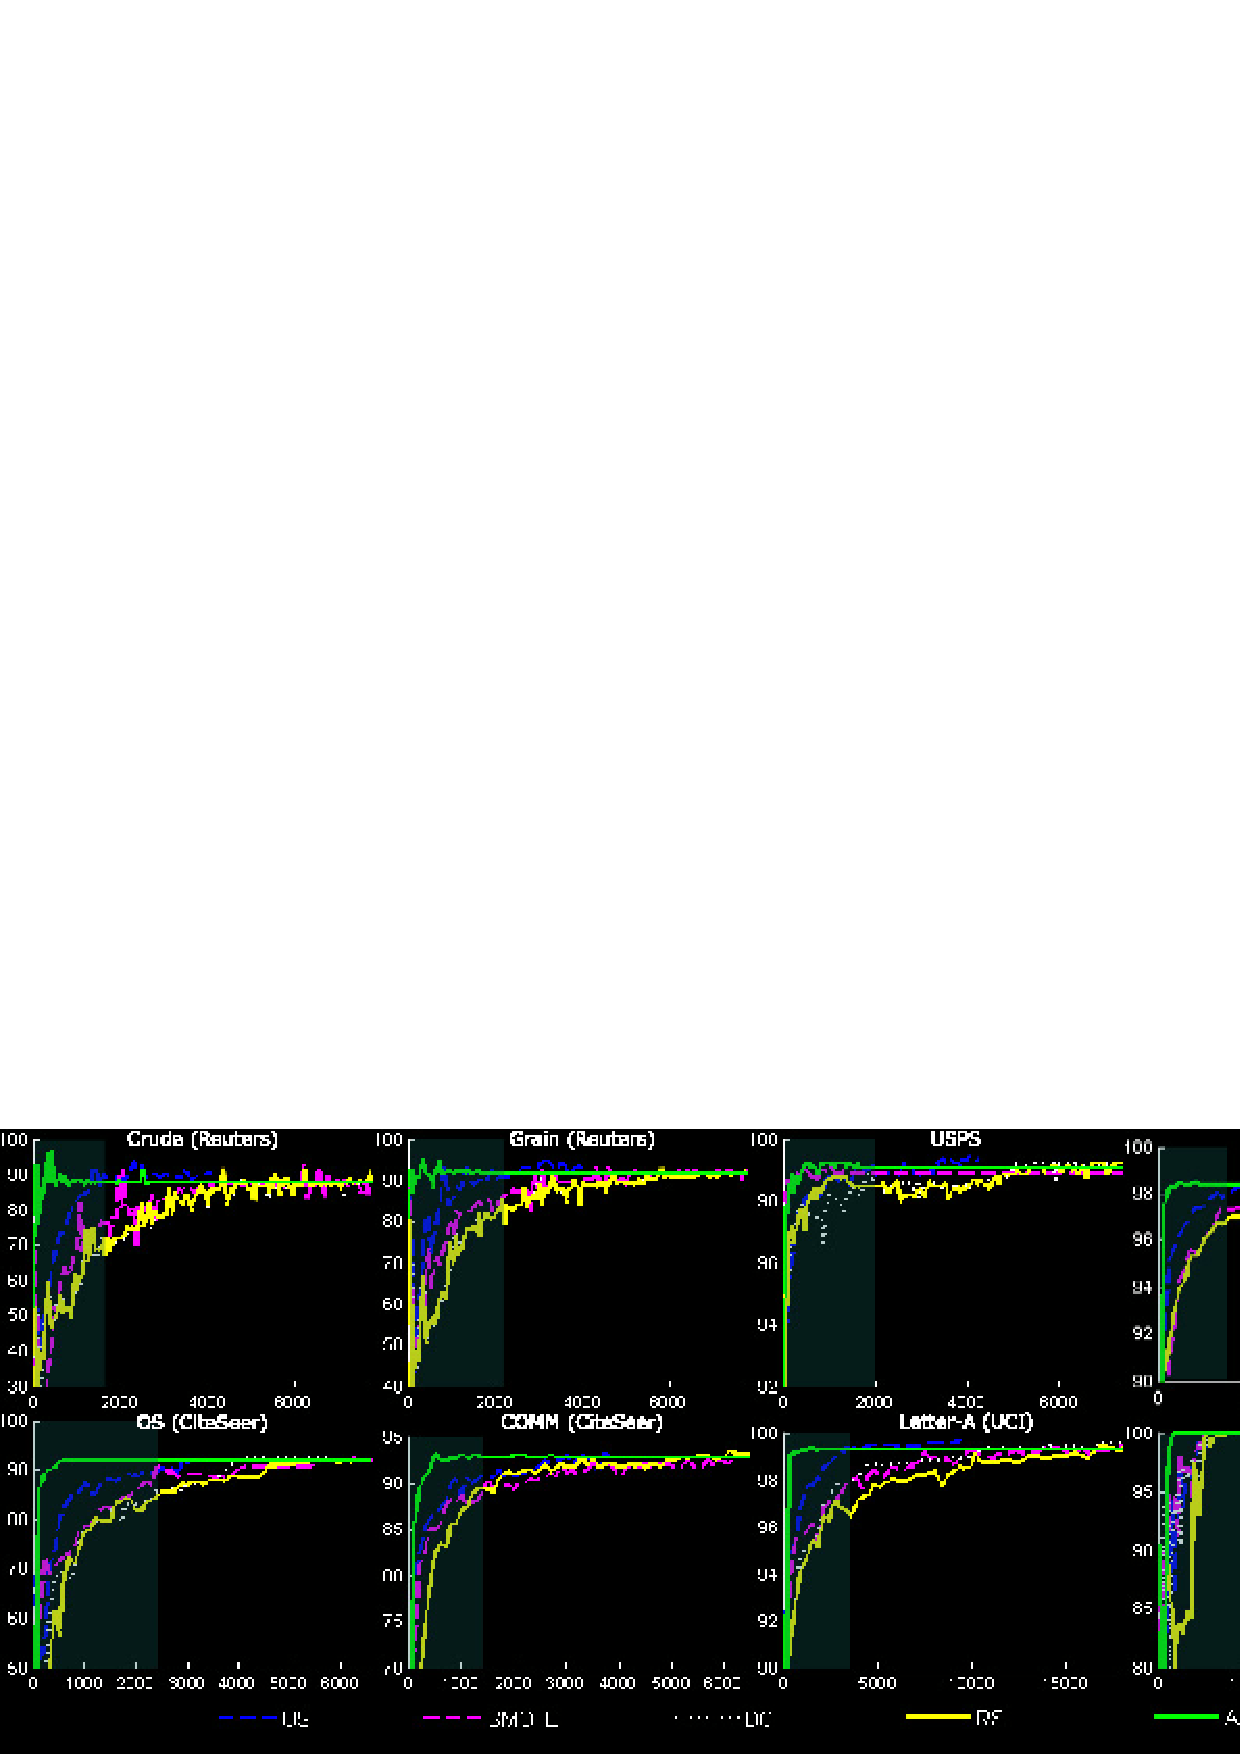
\includegraphics{Figures/lotb/big8.pdf}}
    \caption{Comparisons of g-means. The right border of the shaded area corresponds to the early stopping point.}
    \label{eightgraphs}
\end{figure*}

\begin{table}[!t]\centering \small{
\caption{Comparison of ranks of different methods in PRBEP. The values in bold correspond to the cases where AL win. AL wins in 12 out of 18 cases in PRBEP.}
\begin{tabular}{l|l|c c c c c}
\hline
\multicolumn{2}{c|}{Metric}&\multicolumn{5}{c}{Rank}\\\hline
\multicolumn{2}{c|}{Dataset}&Batch&US&SMOTE&DC&AL\\
\hline\hline
\multirow{5}{5mm}{\begin{sideways}\parbox{13mm}{Reuters}\end{sideways}}
&Corn&1&5&1&4&3\\
&Crude&1&5&1&1&\textbf{1}\\
&Grain&1&5&4&2&2\\
&Interest&2&5&1&3&3\\
&Money-fx&5&4&2&2&\textbf{1}\\
&Ship&4&5&3&1&\textbf{1}\\
&Trade&3&5&3&2&\textbf{1}\\
&Wheat&2&5&2&2&\textbf{1}\\
\hline
\multirow{5}{5mm}{\begin{sideways}\parbox{12mm}{CiteSeer}\end{sideways}}
&AI&4&1&3&5&2\\
&COMM&3&2&3&3&\textbf{1}\\
&CRYPT&1&5&1&1&\textbf{1}\\
&DB&3&2&1&3&3\\
&OS&1&5&1&1&\textbf{1}\\
\hline
\multirow{2}{5mm}{\begin{sideways}\parbox{6mm}{UCI}\end{sideways}}
&Abalone-7&1&1&1&1&\textbf{1}\\
&Letter-A&1&5&4&2&2\\
&Satimage&3&5&3&1&\textbf{1}\\
\hline
\multicolumn{2}{c|}{USPS}&2&2&5&2&\textbf{1}\\
\hline
\multicolumn{2}{c|}{MNIST-8}&3&5&1&3&\textbf{1}\\
\hline
\hline
\multicolumn{2}{c|}{Avg. Rank }&2.28&4.00&2.22&2.17&\textbf{1.50}\\
\hline
\end{tabular}
\label{tbl:rankresults}
}
\end{table}

Since AL involves discarding some instances from the training set, it can be perceived as a type of undersampling method. Unlike US which discards majority samples randomly, AL performs an intelligent search for the most informative ones adaptively in each iteration according to the current hyperplane. In datasets where class imbalance ratio is high such as \emph{corn}, \emph{wheat}, \emph{letter} and \emph{satimage}, we observe significant decrease in PRBEP of US (see Table 3). Note that US's undersampling rate for the majority class in each category is set to the same value as the final support vector ratio which AL reaches in the early stopping point and RS reaches when it sees the entire training data. Although the class imbalance ratio provided to the learner in AL and US are the same, AL achieves significantly better PRBEP performance metric than US. The Wilcoxon signed-rank test (2-tailed) reveals that the zero median hypothesis can be rejected at the significance level 1\% (p=0.0015), implying that AL performs statistically better than US in these 18 datasets. These results reveal the importance of using the informative instances for learning.

Table \ref{tbl:rankresults} presents the rank of PRBEP prediction performance of the five approaches in a variety of datasets. The values in bold correspond to the cases where AL wins and it's clear that winning cases are very frequent for AL (12 out of 18 cases). The average rank also indicates that AL achieves the best PRBEP among the five methods. SMOTE and DC achieve higher PRBEP than the Batch algorithm. The loss of information when undersampling the majority class affects US's prediction performance. Table \ref{tbl:results} also gives the comparison of the computation times of the AL and SMOTE. Note that SMOTE requires significantly long preprocessing time which dominates the training time in large datasets, e.g., MNIST-8 dataset. The low computation cost, scalability and high prediction performance of AL suggest that AL can efficiently handle the class imbalance problem.


%%%%%%%%%%%%%%%%%%%%%%%%
%%%%%%%%%%%%%%%%%%%%%%%%
%%%%%%%%%%%%%%%%%%%%%%%%
%%%%%%%%%%%%%%%%%%%%%%%%
%%%         V     I     R     T     U     A     L          %%%
%%%%%%%%%%%%%%%%%%%%%%%%
%%%%%%%%%%%%%%%%%%%%%%%%
%%%%%%%%%%%%%%%%%%%%%%%%
%%%%%%%%%%%%%%%%%%%%%%%%
%%%%%%%%%%%%%%%%%%%%%%%%


\section{Adaptive Resampling with Active Learning for Imbalanced Data Classification}
\label{virtual}
In Section \ref{lotb_experiments}, our analysis shows the effectiveness of active learning in imbalanced datasets under various data and learner characteristics. One comparison highlighted the benefits over oversampling techniques, and in this section, we present a methodology for using active learning as an oversampling strategy for imbalanced data classification.

In supervised learning, a common strategy to overcome the rarity problem is to resample the original dataset to decrease the overall level of class imbalance. Resampling is done either by oversampling the minority (positive) class and/or undersampling the majority (negative) class until the classes are approximately equally represented \cite{Chawla_2002,Japkowicz_2000,Kubat_1997,Ling_1998}. Oversampling, in its simplest form, achieves a more balanced class distribution either by duplicating minority class instances, or introducing new synthetic instances that belong to the minority class \cite{Chawla_2002}. No information is lost in oversampling since all original instances of the minority and the majority classes are retained in the oversampled dataset. The other strategy to reduce the class imbalance is undersampling, which eliminates some majority class instances mostly by random sampling.

Even though both approaches address the class imbalance problem, they also suffer some drawbacks. The undersampling strategy can potentially sacrifice the prediction performance of the learner, since it is possible to discard informative instances that the learner might benefit. The oversampling strategy, on the other hand, can be overwhelming in case of very large training data. If a complex oversampling method is used, it suffers from high computational costs during preprocessing of the data. Worse yet, oversampling causes longer training time during the learning process due to the increased number of training instances. In addition to suffering from worse runtime performance, it is also inefficient in terms of memory requirements since more instances in addition to the original training data have to be stored. Other costs associated with the learning process (i.e., extended kernel matrix in kernel classification algorithms) are other drawbacks of oversampling.

\subsection{Virtual Instance Resampling Technique Using Active Learning}
In this section, we focus on the oversampling strategy for imbalanced data classification and investigate how it can benefit from the principles of active learning. Our goal is to remedy the efficiency drawbacks of oversampling in imbalanced data classification and use an active learning strategy to generate minority class instances only if they can be useful to the learner. \textsc{Virtual} (Virtual Instance Resampling Technique Using Active Learning)~\cite{Ertekin_dissertation} is a hybrid method of oversampling and active learning that forms an adaptive technique for resampling of the minority class instances. In contrast to traditional oversampling techniques that act as an \textit{offline} step that generate virtual instances of the minority class prior to the training process, \textsc{Virtual} leverages the power of active learning to intelligently and adaptively oversample the data \textit{during} training, removing the need for an offline and separate preprocessing stage. Similar to the discussions in the previous section, \textsc{Virtual} also employs an online SVM-based active learning strategy. In this setting, the informativeness of instances are measured by their distance to their hyperplane, and the most informative instances are selected as the support vectors. \textsc{Virtual} targets the set of support vectors during training, and resamples new instances based on this set. Since most support vectors are found during early stages of training, corresponding virtual examples are also created in the early stages. This prevents the algorithm from creating excessive and redundant virtual instances and integrating the resampling process into the training stage improves the efficiency and generalization performance of the learner compared to other competitive oversampling techniques.

We first briefly discuss the active learning step of the \textsc{Virtual} and explain the virtual instance generation process of the algorithm. We then highlight the advantages of the proposed method.

\subsubsection{Active Selection of Instances}
Let $S$ denote the pool of real and virtual training examples unseen by the learner at each active learning step. Instead of searching for the most informative instance among all the samples in $S$, \textsc{Virtual} queries a randomly picked smaller pool from $S$ based on the ``59 trick'' that we discussed in section \ref{ALpools}. From the small pool, \textsc{Virtual} selects an instance that is closest to the hyperplane according to the current model. If the selected instance is a real positive instance (from the original training data) and becomes a support vector, \textsc{Virtual} advances to the oversampling step, which we explain in the following section. Otherwise, the algorithm proceeds to the next iteration to select another instance.


\begin{algo}[!b]
\begin{center} \small
\begin{tabular}{l}
{\bfseries Define:} \\
~~$X=\{x_1, x_2, \cdots, x_n\}$ : training instances \\
~~$X^+_{R}$ : positive real training instances\\
~~$S$ : pool of training instances for SVM\\
~~$v$ : \# virtual instances to create in each iteration\\
~~$L$ : size of the small set of randomly picked samples\\
~~~~~~~ for active sample selection\\
\hline
\\
1.~~Initialize $S \leftarrow X$\\
2.~~{\bfseries while} $S \neq \emptyset$\\
3.~~~~~~//~\textit{Active sample selection step}\\
4.~~~~~~$d_{min}\leftarrow \infty$\\
5.~~~~~~{\bfseries for} $i \leftarrow 1$ to $L$\\
6.~~~~~~~~~~$x_j \leftarrow RandomSelect(S)$\\
7.~~~~~~~~~~{\bfseries If} $d(x_j, hyperplane) < d_{min}$\\
8.~~~~~~~~~~~~~~$d_{min}\leftarrow d(x_j, hyperplane)$\\
9.~~~~~~~~~~~~~~$candidate \leftarrow x_j$\\
10.~~~~~~~~~{\bfseries end}\\
11.~~~~~{\bfseries end}\\
12.~~~~~$x_s \leftarrow candidate$\\
13.~~~~~//~\textit{Virtual Instance Generation}\\
14.~~~~~{\bfseries If} $x_s$ becomes SV {\bfseries and} $x_s \in X^+_{R}$\\
15.~~~~~~~~~$K \leftarrow$ $k$ nearest neighbors of $x_s$\\
16.~~~~~~~~~{\bfseries for} $i \leftarrow 1$ to $v$\\
17.~~~~~~~~~~~~~$x_m \leftarrow RandomSelect(K)$\\
18.~~~~~~~~~~~~~//~Create a virtual positive instance $x^v_{s,m}$ between $x_s$ and $x_m$ \\
19.~~~~~~~~~~~~~$\lambda$=random number between 0 and 1\\
20.~~~~~~~~~~~~~$x^v_{s,m} = \lambda \cdot x_s + (1-\lambda)x_m$\\
21.~~~~~~~~~~~~~$S \leftarrow S \cup x^v_{s,m}$\\
22.~~~~~~~~~{\bfseries end}\\
23.~~~~~{\bfseries end}\\
24.~~~~~$S \leftarrow S - x_s$\\
25.~{\bfseries end}
\vspace{-3mm}
\end{tabular}
\end{center}
\caption{VIRTUAL}
\label{algo_virtual}
\end{algo}

\subsubsection{Virtual Instance Generation}
\textsc{Virtual} oversamples the real minority class instance (from the original training data) which become a support vector in the current iteration. It selects the $k$ nearest minority class neighbors $(x_{i\rightarrow 1} \cdots x_{i \rightarrow k})$ of $x_i$ based on their similarities in the kernel transformed higher dimensional feature space. We limit the neighboring instances of $x_i$ to the minority class so that the new virtual instances lie within the minority class distribution. Depending on the amount of over-sampling required, the algorithm creates $v$ virtual instances. Each virtual instance lies on any of the line segments joining $x_i$ and its neighbor $x_{i\rightarrow j}\ (j=1,...,k)$. In other words, a neighbor $x_{i \rightarrow j}$ is randomly picked and the virtual instance is created as $\bar{x}_v = \lambda \cdot x_i + (1-\lambda)x_{i \rightarrow j}$,  where $\lambda\in(0,1)$ determines the placement of $\bar{x}_v$ between $x_i$ and $x_{i \rightarrow j}$. All $v$ virtual instances are added to $S$ and are eligible to be picked by the active learner in the subsequent iterations.

The pseudocode of \textsc{Virtual} given in Algorithm \ref{algo_virtual}  depicts the two processes described above. In the beginning, the pool $S$ contains all real instances in the training set. At the end of each iteration, the instance selected is removed from $S$, and any virtual instances generated are included in the pool $S$. In this pseudocode, \textsc{Virtual} terminates when there are no instances in $S$. In Section \ref{early_stop}, we propose an early stopping criteria for \textsc{Virtual}.

\begin{figure*}[t!bp]
  \begin{center}
     \mbox{
      \subfigure[Oversampling with SMOTE]{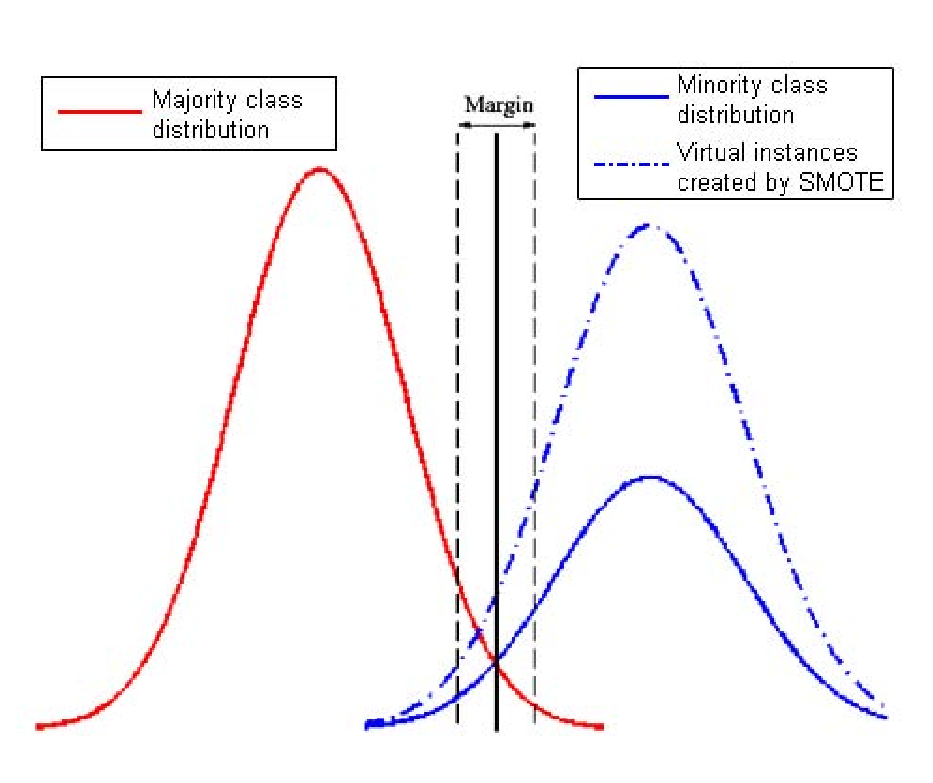
\includegraphics[width=0.45\textwidth, height=4.2cm]{Figures/virtual/smote_proc.eps}
      \label{fig:smote_sample}
      } \quad
      \subfigure[Oversampling with \textsc{Virtual}]{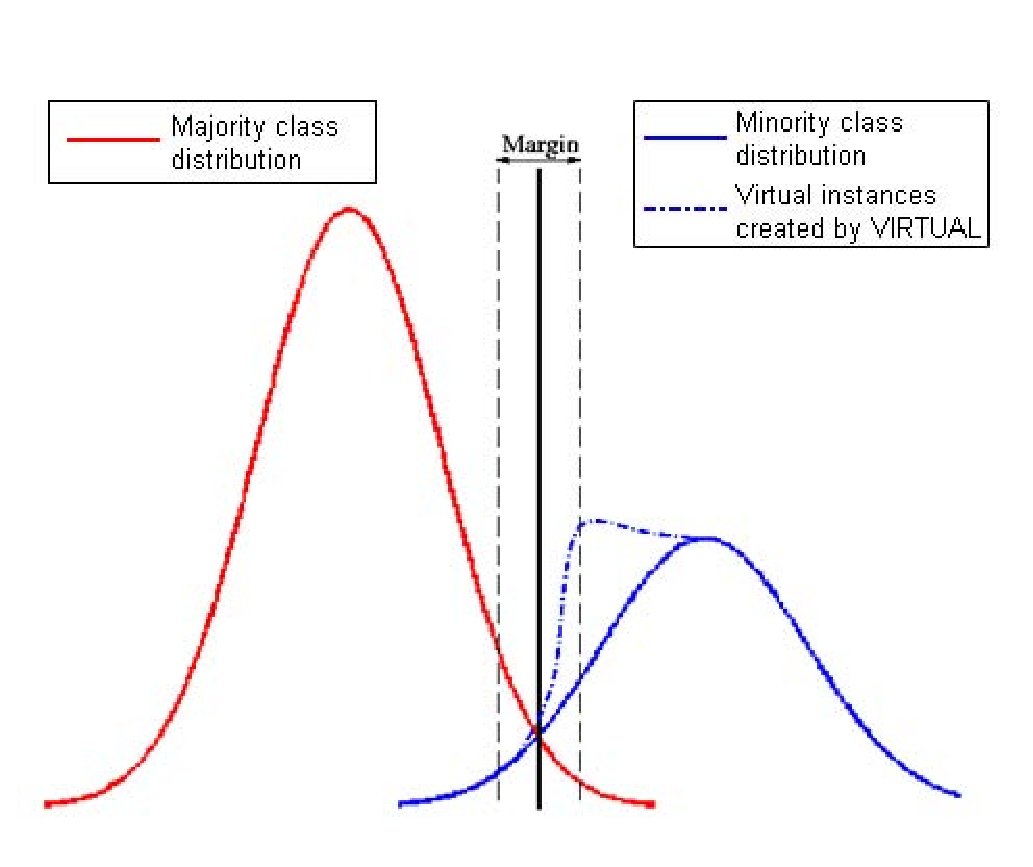
\includegraphics[width=0.45\textwidth, height=4.2cm]{Figures/virtual/virtual_proc.eps}
      \label{fig:virtual_sample}
      }
      }
    \caption{Comparison of oversampling the minority class with SMOTE and VIRTUAL. }
    \label{fig:oversample}
  \end{center}
\end{figure*}

\subsection{Remarks on VIRTUAL}
We compare \textsc{Virtual} with a popular oversampling technique SMOTE to  illustrate the advantages of the proposed algorithm. Figure \ref{fig:oversample} shows the different behavior of how SMOTE and \textsc{Virtual} create virtual instances for the minority class. SMOTE creates virtual instance(s) for each positive example (see Figure \ref{fig:smote_sample}), whereas \textsc{Virtual} creates the majority of virtual instances around the positive canonical hyperplane (shown with a dashed line in Figure \ref{fig:virtual_sample}). Note that a large portion of virtual instances created by SMOTE are far away from the hyperplane and thus are not likely to be selected as support vectors. \textsc{Virtual}, on the other hand, generates virtual instances near the real positive support vectors adaptively in the learning process. Hence the virtual instances are near the hyperplane and thus are more informative.

We further analyze the computation complexity of SMOTE and \textsc{Virtual}.  The computation complexity of \textsc{Virtual} is $O(\left|SV(+) \right|\cdot v \cdot \mathcal{C})$, where $v$ is the number of virtual instances created for a real positive support vector in each iteration, $\left|SV(+) \right|$ is the number of positive support vectors and $\mathcal{C}$ is the cost of finding k nearest neighbors. The computation complexity of SMOTE is $O(\left| X_R^+\right| \cdot v \cdot \mathcal{C})$, where $\left| X_R^+\right|$ is the number of positive training instances. $\mathcal{C}$ depends on the approach for finding k nearest neighbors. The naive implementation searches all $N$ training instances for the nearest neighbors and thus $\mathcal{C}=kN$. Using advanced data structure such as kd-tree, $\mathcal{C}=k\log N$. Since $\left|SV(+) \right|$ is typically much less than $\left| X_R^+\right|$, \textsc{Virtual} incurs lower computation overhead than SMOTE. Also, with fewer virtual instances created, the learner is less burdened with \textsc{Virtual}. We demonstrate with empirical results that the virtual instances created with \textsc{Virtual} are more informative and the prediction performance is also improved.

\subsection{Experiments}
We conduct a series of experiments both on synthetic and real-world datasets to demonstrate the efficacy of \textsc{Virtual}. We compare \textsc{Virtual} with two systems, Active Learning (AL) and SMOTE. AL solely adopts the traditional active learning strategy without preprocessing or creating any virtual instances during learning. SMOTE, on the other hand, preprocesses the data by creating virtual instances before training and uses random sampling in learning. Experiments elicit the advantages of adaptive virtual sample creation in \textsc{Virtual}.

\begin{figure}[b!]
\begin{center}
\hspace{-10mm}
\subfigure {
\includegraphics[width=40mm]{Figures/virtual/wf_imb_rt_1.jpg}
}
\subfigure {
\includegraphics[width=40mm]{Figures/virtual/wf_imb_rt_2.jpg}
}
\subfigure {
\includegraphics[width=40mm]{Figures/virtual/wf_imb_rt_3.jpg}
} \\
\hspace{-10mm}
\subfigure {
\includegraphics[width=40mm]{Figures/virtual/wf_imb_rt_4.jpg}
}
\subfigure {
\includegraphics[width=40mm]{Figures/virtual/wf_imb_rt_5.jpg}
}
\subfigure {
\includegraphics[width=40mm]{Figures/virtual/wf_imb_rt_legend.jpg}
}
\end{center}
  \caption{Comparison of Active Learning and VIRTUAL on the \emph{Waveform} dataset with
  different imbalance ratios (Imb.R.=2, 4, 8, 16, 32). The test results are average of ten runs.}
  \label{fig:waveform}
\end{figure}


\subsubsection{Simulation Study}\label{early_stop}
The popular waveform example is widely used in classification literature \cite{Breiman84}. In this example, three shifted triangular waveforms
\begin{eqnarray*}
v_1(j)&=&max(6-|j-11|,0)\\
v_2(j)&=&v_1(j-4)\\
v_3(j)&=&v_1(j+4)
\end{eqnarray*}
are linearly combined into 21 variables:
\[
x_j  = \left\{ \begin{array}{l}
 u \cdot v_1 (j) + (1 - u)v_2 (j) + \varepsilon _j,\ \mbox{Class 1}  \\
 u \cdot v_1 (j) + (1 - u)v_3 (j) + \varepsilon _j,\ \mbox{Class 2}  \\
 u \cdot v_2 (j) + (1 - u)v_3 (j) + \varepsilon _j,\ \mbox{Class 3} \\
 \end{array} \right.
\]
where $ j=1,2,...,21$, $u$ is uniformly distributed on $(0,1)$ and $\varepsilon _j$ is the normal Gaussian noise. In our case, we use samples from Class 1 as positive samples and the others as negative and thus the imbalance ratio is 2. We randomly draw 4,000 samples for training and independently draw 1,000 samples for testing.

To showcase the different behavior of AL and \textsc{Virtual} in different imbalance ratio (Imb.R.) data, we undersample the positive class to obtain five datasets (\emph{Waveform} Imb.R.= $2^1, 2^2, 2^3, 2^4, 2^5$). Figure \ref{fig:waveform} demonstrates the g-means of AL and \textsc{Virtual} in these five datasets. We observe that when data is moderately imbalanced (Imb.R.=2, 4), the g-means curves of the two methods are close to each other. When the imbalance ratio increases, the g-means of AL drops faster than that of \textsc{Virtual} and thus the gap widens. In the \emph{Waveform} Imb.R. 32 dataset, there are 83 positive instances and AL uses them all as support vectors. Since \textsc{Virtual} (v=1) creates a virtual instance for each real positive support vector, it creates 83 positive virtual instances and most of them are selected as support vectors (see Figure \ref{fig:waveform-sv}). As a result, the number of positive support vectors nearly doubles and the number of positive and negative support vectors is more balanced. Figure \ref{fig:waveform} compares the g-means of AL and \textsc{Virtual} for different class imbalance ratios and illustrates that these adaptively created positive training instances in \textsc{Virtual} contribute to the improvement in g-means over AL. Therefore, \textsc{Virtual} is shown to be more resilient to imbalanced data.

\begin{figure*}[t!]
  \begin{center}
     \mbox{
      \subfigure[Number of support vectors in VIRTUAL versus number of training instances in \emph{Waveform} (Imb.R.=32)]{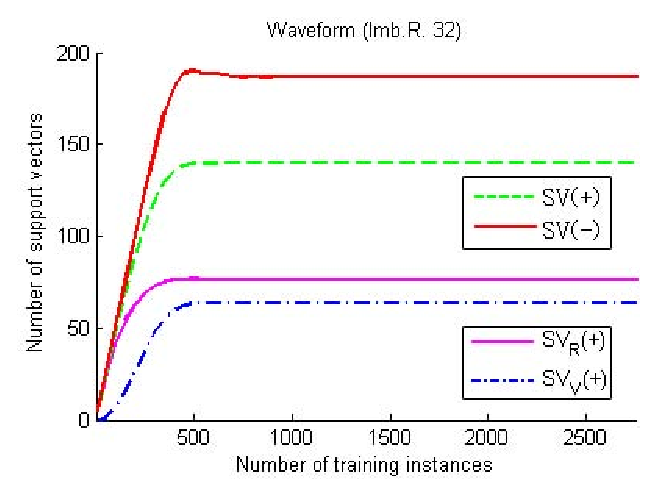
\includegraphics[width=0.47\textwidth, height=3.9cm]{Figures/virtual/wf-32sv-proc.eps}
      \label{fig:waveform-sv}
      } \quad
      \subfigure[Saturation of number of support vectors and g-means for \emph{Waveform} (Imb.R.=4). The vertical line indicates where support vectors saturate and training stops.]{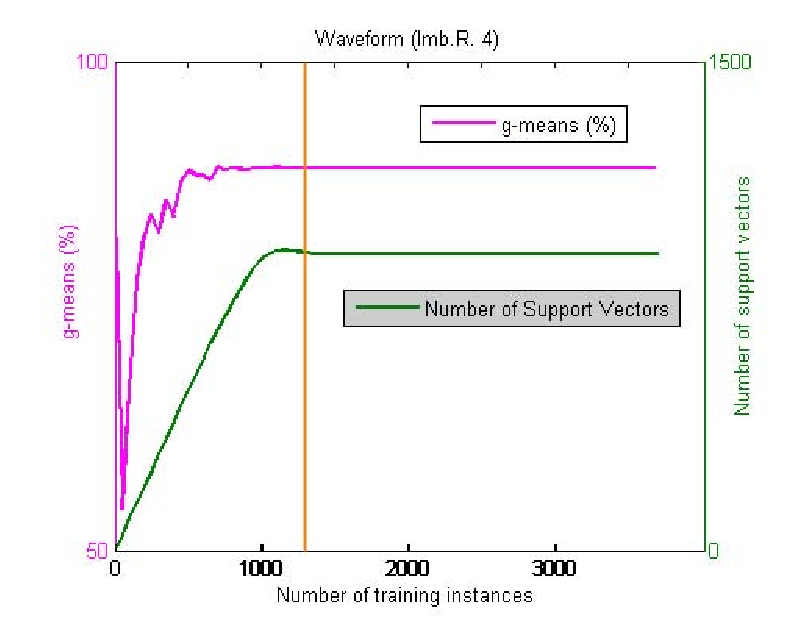
\includegraphics[width=0.47\textwidth, height=3.9cm]{Figures/virtual/wf4-sv.eps}
      \label{fig:waveform-sv-gmeans}
      }
      }
    \caption{Growth of the number of support vectors for \emph{Waveform}}
    \label{fig:waveform-sv-all}
  \end{center}
\end{figure*}

Figure \ref{fig:waveform-sv} further unpacks the adaptive learning process of \textsc{Virtual} in the \emph{Waveform} Imb.R. 32 dataset. When the first 150 training instances are seen, the number of real positive support vectors ($SV_R(+)$) and negative support vectors ($SV(-)$) is balanced. This effect is due to the active learning strategy, because in early iterations active learning picks positive and negative samples in a balanced manner whereas random sampling selects examples proportional to the data imbalance ratio. In this stage, the number of virtual positive instances is relatively small
compared to the real positive instances and thus few are selected into the model. Later, the real positive samples are selected more slowly (deviating from the straight line) and they are eventually exhausted. During this stage, virtual positive instances continue to be created and a large portion of them are selected into the model. Finally, the model becomes saturated using only 500 of the original total 2,757 training instances. By creating virtual examples, \textsc{Virtual} nearly doubles the number of positive support vectors and thus the support vector ratio becomes more balanced. As seen in Figure \ref{fig:waveform}, the adaptively created virtual examples help to guide the learner to achieve better g-means. This experiments on artificial dataset demonstrates the superiority of \textsc{Virtual} over AL in more imbalanced datasets.

In Figure \ref{fig:waveform-sv-gmeans}, we observe that when the number of support vectors saturates g-means also stabilizes. Seeing additional instances after a point does not change the model, as the
training instances in the margin are exhausted. Accordingly, we apply an early stopping criteria to eliminate the learning stage which has little, if any, impact on the prediction performance. A theoretically sound method to stop training is to check if there are still unseen training instances in the margin, the distance of the newly selected instance is compared to the support vectors of the current model. If the new selected instance by active learning (closest to the hyperplane) is not closer than any of the support vectors, we conclude that the margin is exhausted. A practical implementation of this idea is to count the number of support vectors during the active learning process.  If the number of the support vectors stabilizes, it implies that all possible support vectors have been selected into the model. Early stopping shortens the training time without sacrificing prediction performance. We adopt this strategy in our experiments to find the early stopping points where active learning is used.

\begin{table}[ht] \small
\caption{The Reuters and 4 UCI datasets.} \centering
\begin{tabular}{l|l|c@{\hspace{2mm}}r@{\hspace{2mm}}r@{\hspace{2mm}}c}
\hline
\multicolumn{2}{c|}{Dataset}&\#Feature&\#Pos&\#Neg&Imb. Ratio\\
\hline\hline
\multirow{10}{2mm}{\begin{sideways}\parbox{13mm}{Reuters}\end{sideways}}
&acq&8315&1650&6120&3.7\\
&corn&8315&181&7589&41.9\\
&crude&8315&389&7381&19.0\\
&earn&8315&2877&4893&1.7\\
&grain&8315&433&7337&16.9\\
&interest& 8315 &347&7423&21.4\\
&money-fx& 8315 &538&7232&13.4\\
&ship& 8315 &197&7573&38.4\\
&trade&8315&369&7401&20.1\\
&wheat& 8315 &212&7558&35.7\\
\hline\hline
\multirow{4}{2mm}{\begin{sideways}\parbox{5mm}{UCI}\end{sideways}}
&abalone&9&352&3407&9.7\\
&breast&9&172&320&1.9\\
&letter&16&710&17290&24.4\\
&satimage&36&415&4020&9.7\\
\hline
\end{tabular}
\label{tbl:virtual_datasets}
\end{table}

\subsubsection{Experiments on Real-World Data}
We study the performance of the algorithm on real-world data using several benchmark datasets. On the \emph{Reuters-21578} dataset, we test the algorithms with the top 10 most populated categories. In each category relevant instances are labeled as positive and the remaining as negative. We also used 4 benchmark datasets from the popular UCI Machine Learning Repository. \emph{Letter} and \emph{satimage} are image datasets. The `letter A' is used as the positive class in \emph{letter} and `class 4' (damp grey soil) is used as positive class in \emph{satimage}. \emph{Abalone} and \emph{Wisconsin breast cancer} (\emph{breast}) are biology and medical diagnosis datasets respectively. In \emph{abalone}, instances labeled as `class 7' form the positive class and instances labeled as `m.o.ant' constitute the positive class in \emph{breast}. These datasets cover a wide range of data imbalance ratio (see Table \ref{tbl:virtual_datasets}).

\begin{figure*}[!b]
  \centering
  \scalebox{1}
  {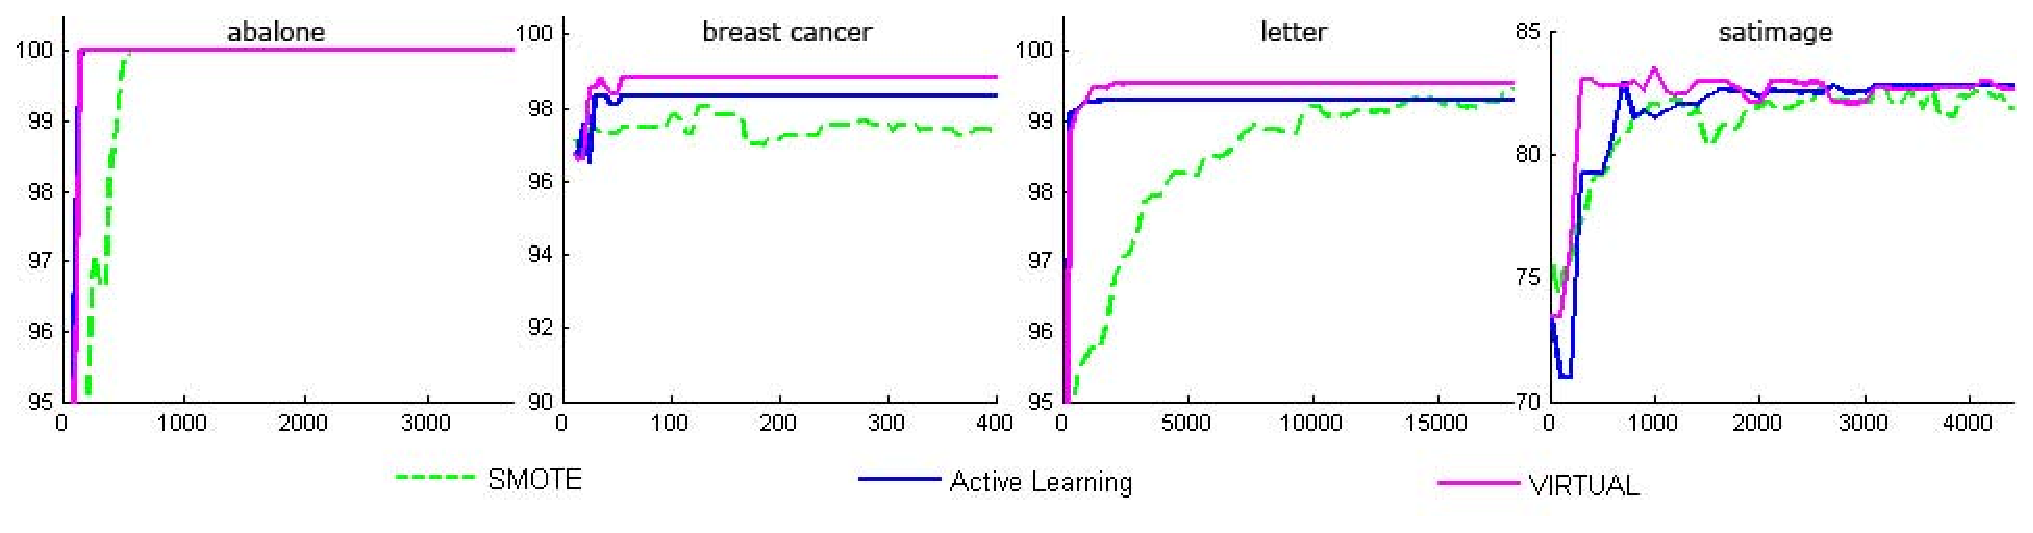
\includegraphics[width=\textwidth]{Figures/virtual/uci-graphs.eps}}\\
  \caption{Comparison of SMOTE, AL and VIRTUAL on \emph{UCI} datasets.
  We present the g-means (\%) (y-axis) of the current model for the test set
  vs. the number of training samples (x-axis) seen.}
  \label{fig:uci}
\end{figure*}

\begin{figure*}[!b]
  \centering
  \scalebox{1}
  {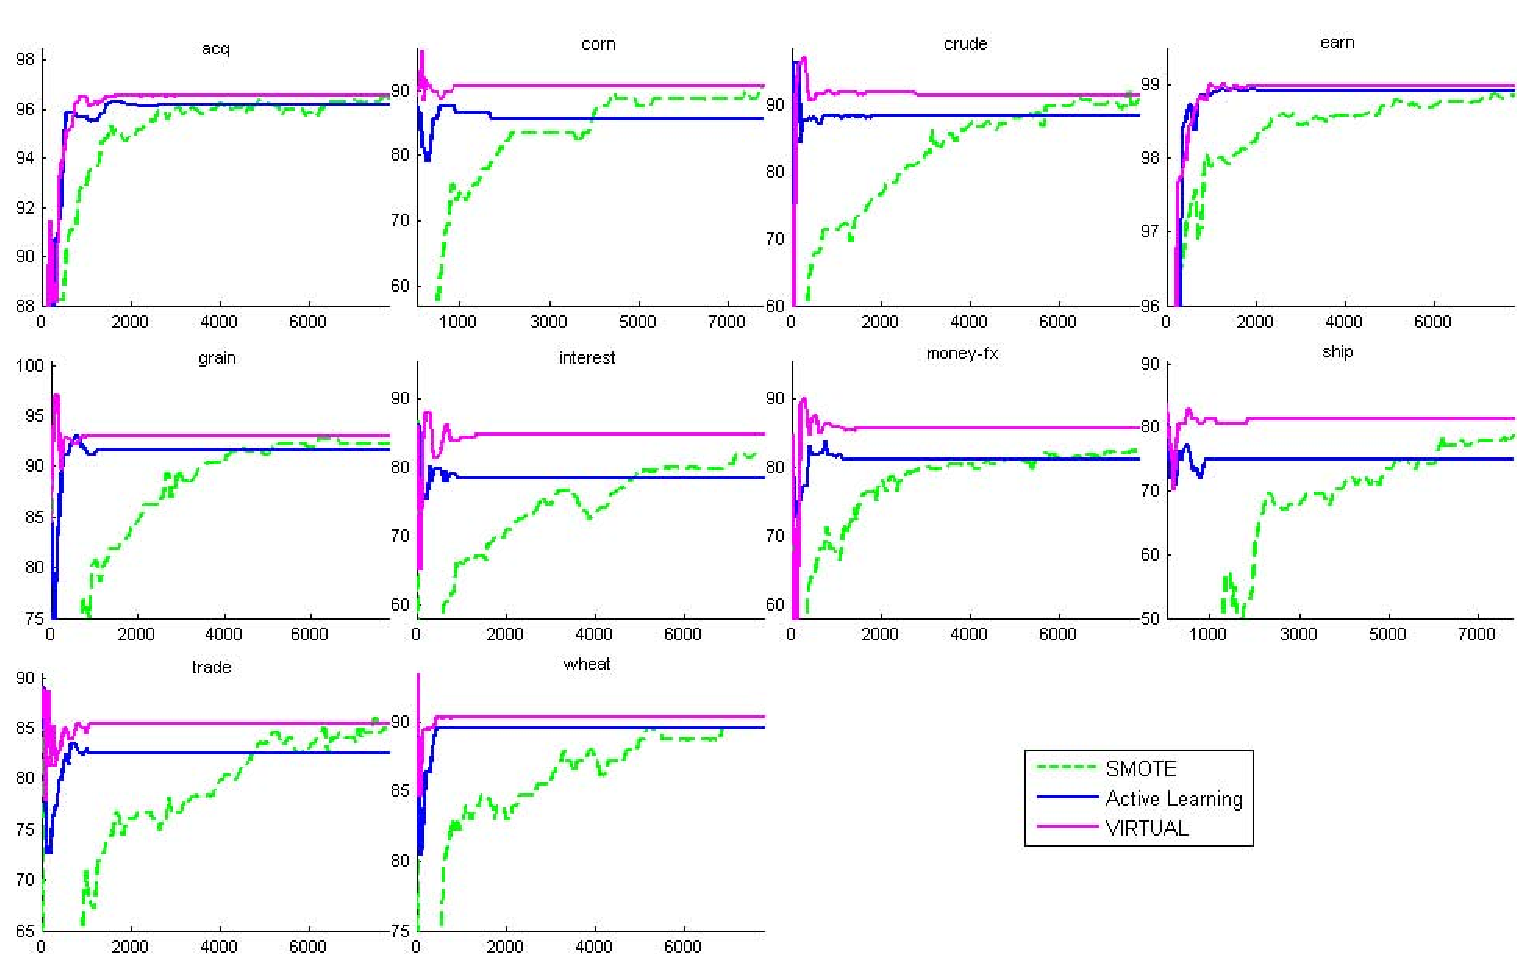
\includegraphics[width=\textwidth]{Figures/virtual/reuters.eps}}\\
  \caption{Comparison of SMOTE, AL and VIRTUAL on 10 largest categories of \emph{Reuters-21578}.
  We show the g-means (\%) (y-axis) of the current model for the test set
  versus the number of training samples (x-axis) seen.}
  \label{fig:reuters}
\end{figure*}

In Figures \ref{fig:uci} and \ref{fig:reuters},  we provide the details on the behavior of the three algorithms, SMOTE, AL and \textsc{Virtual}. For the Reuters datasets (Figure \ref{fig:reuters}), we note that in all the 10 categories \textsc{Virtual} outperforms AL in g-means metric after saturation. The difference in performance is most pronounced in the more imbalanced categories, e.g. \emph{corn}, \emph{interest} and \emph{ship}. In the less imbalanced datasets such as \emph{acq} and \emph{earn}, the difference in g-means of both methods is less noticeable. The g-means of SMOTE converges much slower than both AL and \textsc{Virtual}. However, SMOTE converges to higher g-means than AL in some of the categories, indicating that the virtual positive examples provide additional information that can be used to improve the model. \textsc{Virtual} converges to the same or even higher g-means than SMOTE while generating fewer virtual instances. For the UCI datasets (Figure \ref{fig:uci}), \textsc{Virtual} performs as well as AL in \emph{abalone} in g-means and consistently outperforms AL and SMOTE in the other three datasets.
\begin{table}[!t]
\centering \small
\caption{Support vectors with SMOTE (SMT), AL and VIRTUAL. Imb.Rt. is the data imbalance ratio and
\#SV(-)/\#SV(+) represents the support vector imbalance ratio. The rightmost two columns compare the portion of the virtual instances selected as support vectors in SMOTE and VIRTUAL.}
\small
\begin{tabular}{l@{\hspace{1mm}}|l@{\hspace{1mm}}|c@{\hspace{1mm}}|c@{\hspace{1mm}}|c@{\hspace{1mm}}|c@{\hspace{1mm}}|c@{\hspace{1mm}}|c}
\hline
\multicolumn{2}{c|}{\multirow{2}{1cm}{Dataset}}&Imb.&\multicolumn{3}{c|}{\#SV(-)/\#SV(+)}&\multicolumn{2}{c}{\#$SV_V(+)$/\#V.I.}\\\cline{4-8}
\multicolumn{2}{c|}{}&Rt.&SMT&AL&\textsc{Virtual}&SMT&\textsc{Virtual}\\
\hline\hline
\multirow{10}{2mm}{\begin{sideways}\parbox{13mm}{Reuters}\end{sideways}}
&acq&3.7&1.24&1.28&1.18&2.4\%&\textbf{20.3\%}\\
&corn&41.9&2.29&3.08&1.95&17.1\%&\textbf{36.6\%}\\
&crude&19.0&2.30&2.68&2.00&10.8\%&\textbf{50.4\%}\\
&earn&1.7&1.68&1.89&1.67&6.0\%&\textbf{24.2\%}\\
&grain&16.9&2.62&3.06&2.32&7.2\%&\textbf{42.3\%}\\
&interest&21.4&1.84&2.16&1.66&13.3\%&\textbf{72.2\%}\\
&money-fx&13.4&1.86&2.17&1.34&8.2\%&\textbf{31.1\%}\\
&ship&38.4&3.45&4.48&2.80&20.0\%&\textbf{66.5\%}\\
&trade&20.1&1.89&2.26&1.72&15.4\%&\textbf{26.6\%}\\
&wheat&35.7&2.55&3.43&2.22&12.3\%&\textbf{63.9\%}\\
\hline\hline
\multirow{4}{2mm}{\begin{sideways}\parbox{5mm}{UCI}\end{sideways}}
&abalone&9.7&0.99&1.24&0.99&30.4\%&\textbf{69.2\%}\\
&breast&1.9&1.23&0.60&0.64&2.9\%&\textbf{39.5\%}\\
&letter&24.4&1.21&1.48&0.97&0.98\%&\textbf{74.4\%}\\
&satimage&9.7&1.31&1.93&0.92&37.3\%&\textbf{53.8\%}\\
\hline
\end{tabular}
\label{tbl:res_svs}
\end{table}

In Table \ref{tbl:res_svs}, the support vector imbalance ratio of all the three methods are lower than the data imbalance ratio, and \textsc{Virtual} achieves the most balanced ratios of positive and negative support vectors in the Reuters datasets. Despite that the datasets we used have different data distributions, the portion of virtual instances which become support vectors in \textsc{Virtual} consistently and significantly higher than that in SMOTE. These results confirm our previous discussion that \textsc{Virtual} is more effective in generating informative virtual instances.

Table \ref{tbl:res_all} presents g-means and the total learning time for SMOTE, AL and  \textsc{Virtual}. Classical batch SVM's g-means values are also provided as a reference point. In Reuters datasets, \textsc{Virtual} yields the highest g-means in all categories. Table 4 shows the effectiveness of adaptive virtual instance generation. In categories \emph{corn}, \emph{interest} and \emph{ship} with high class imbalance ratio, \textsc{Virtual} gains substantial improvement in g-means. Compared to AL, \textsc{Virtual} requires additional time for the creation of virtual instances and selection of those which may become support vectors. Despite this overhead, \textsc{Virtual}'s training times are comparable with that of AL. In the cases where minority examples are abundant, SMOTE demands substantially longer time to create virtual instances than \textsc{Virtual}. But as the rightmost columns in Table 3 show, only a small fraction of the virtual instances created by SMOTE become support vectors. Therefore SMOTE spends much time to create virtual instances that will not be used in the model. On the other hand, \textsc{Virtual} has already a short training time and uses this time to create more informative virtual instances. In Table 4, the numbers in parentheses give the ranks of the g-means prediction performance of the four approaches. The values in bold correspond to a win and \textsc{Virtual} wins in nearly all datasets.  The Wilcoxon signed-rank test (2-tailed) between \textsc{Virtual} and its nearest competitor SMOTE reveals that the zero median hypothesis can be rejected at the significance level 1\% ($p=4.82 \times 10^{-4}$), implying that \textsc{Virtual} performs statistically better than SMOTE in these 14 datasets. These results reveal the importance of creating synthetic samples from the informative instances rather than all the instances.


\begin{table*}[!tp]\centering \small
\caption{g-means and total learning time using SMOTE, AL and VIRTUAL.
`Batch' corresponds to the classical SVM learning in batch setting without resampling.
The numbers in brackets denote the rank of the corresponding method in the dataset.}
\begin{tabular}{l|l|c@{\hspace{1mm}}|c@{\hspace{1mm}}|c@{\hspace{1mm}}|c@{\hspace{1mm}}|c|r|c}
\hline
\multicolumn{2}{c|}{\multirow{2}{1cm}{Dataset}}&\multicolumn{4}{c|}{g-means (\%)}&\multicolumn{3}{c}{Total learning time (sec.)}\\\cline{3-9}
\multicolumn{2}{c|}{}&Batch&SMOTE&AL&\textsc{Virtual}&SMOTE&AL&\textsc{Virtual}\\
\hline\hline
\multirow{10}{3mm}{\begin{sideways}\parbox{13mm}{Reuters}\end{sideways}}
&acq&96.19 (3)&96.21 (2)&96.19 (3)&\textbf{96.54 (1)}&2271&146&203\\
&corn&85.55 (4)&89.62 (2)&86.59 (3)&\textbf{90.60 (1)}&74&43&66\\
&crude&88.34 (4)&91.21 (2)&88.35 (3)&\textbf{91.74 (1)}&238&113&129\\
&earn&98.92 (3)&\textbf{98.97 (1)}&98.92 (3)&\textbf{98.97 (1)}&4082&121&163\\
&grain&91.56 (4)&92.29 (2)&91.56 (4)&\textbf{93.00 (1)}&296&134&143\\
&interest&78.45 (4)&83.96 (2)&78.45 (4)&\textbf{84.75 (1)}&192&153&178\\
&money-fx&81.43 (3)&83.70 (2)&81.08 (4)&\textbf{85.61 (1)}&363&93&116\\
&ship&75.66 (3)&78.55 (2)&74.92 (4)&\textbf{81.34 (1)}&88&75&76\\
&trade&82.52 (3)&84.52 (2)&82.52 (3)&\textbf{85.48 (1)}&292&72&131\\
&wheat&89.54 (3)&89.50 (4)&89.55 (2)&\textbf{90.27 (1)}&64&29&48\\
\hline\hline
\multirow{4}{2mm}{\begin{sideways}\parbox{5mm}{UCI}\end{sideways}}
&abalone&\textbf{100 (1)}&\textbf{100 (1)}&\textbf{100 (1)}&\textbf{100 (1)}&18&4&6\\
&breast&98.33 (2)&97.52 (4)&98.33 (2)&\textbf{98.84 (1)}&4&1&1\\
&letter&99.28 (3)&99.42 (2)&99.28 (3)&\textbf{99.54 (1)}&83&5&6\\
&satimage&\textbf{83.57 (1)}&82.61 (4)&82.76 (3)&82.92 (2)&219&18&17\\
\hline
\end{tabular}
\vspace{-3mm}
\label{tbl:res_all}
\end{table*}

\drop{
\section{Conclusions}
The class imbalance problem has been known to hinder the generalization performance of classification algorithms. This chapter offers a better understanding of how active learning can remedy the problems that stem from class imbalance and presents techniques to improve the efficiency of active learning when dealing with such problems.

In the first part of the chapter, we first present an efficient active learning method which selects informative instances from a randomly picked small pool of examples rather than making a full search in the entire training set. This strategy renders active learning to be applicable to very large datasets which otherwise would be computationally very expensive. Combined with the early stopping heuristics, active learning achieves a fast and scalable solution without sacrificing prediction performance. We then show that this active learning strategy can be used to address the class imbalance problem. In simulation studies, we demonstrate that as the imbalance ratio increases, active learning can achieve better prediction performance than random sampling by only using the informative portion of the training set. By focusing the learning on the instances around the classification boundary, more balanced class distributions can be provided to the learner in the earlier steps of the learning.  Our empirical results on a variety of real-world datasets allow us to conclude that active learning is comparable or even better than other popular resampling methods in dealing with imbalanced data classification.

The second part presents an active learning based adaptive resampling strategy, \textsc{Virtual} to address the imbalanced data classification problem in SVMs. \textsc{Virtual} adaptively creates instances according to the real positive support vectors selected in each active learning step. These instances are informative as they are close to the hyperplane. Thus \textsc{Virtual} creates fewer virtual instances that are informative. Our complexity analysis shows that \textsc{Virtual} incurs lower overhead in data generation and eventually less burden to the learner. Our thorough empirical results on both artificial and real-world data demonstrate that \textsc{Virtual} is capable of
achieving higher g-means than active learning without oversampling (AL) and SMOTE. Experimental results also show that \textsc{Virtual} is more resilient to high class imbalance ratios due to its capability of creating more balanced models using the virtual instances created. The training time of \textsc{Virtual} is substantially shorter than SMOTE in most cases.
}
